\documentclass[12pt]{ULrapport}
\usepackage[utf8]{inputenc}
\usepackage[french]{babel}
\usepackage{float}
\restylefloat{table}
\usepackage{hhline}
\usepackage{pdfpages}
\usepackage{hyperref}
\usepackage{lscape}
\usepackage{pdflscape}




% Title Page
\title{Design 3}
\author{Name 1, Name 2, Rémi Mercier, Name 4}



\TitreProjet{Pirates des Caraïbes}
\TitreRapport{Rapport de développement}
\Destinataire{Dominique Grenier, Philippe Giguère, Denis Laurendeau}
\NumeroEquipe{4}
%\NomEquipe{Équipe 1}
\TableauMembres{%
	111\,076\,721  & Mercier, Rémi     & \\\hline
	111\,076\,680  & Bilodeau, Dominic     & \\\hline
	111\,073\,278  & Béland, Camille     & \\\hline
	111\,040\,716  & Arel, David     & \\\hline
	111\,096\,321  & B. Bolduc, Adam     & \\\hline
	111\,075\,609  & Lévesque, Mathieu    & \\\hline
	908\,188\,831  & Papillon, Maxime  & \\\hline
	907\,152\,804  & Jean-Christophe Martin-Morin & \\\hline
}
\DateRemise{28 février 2016}
% Contenu de l'historique des versions
\HistoriqueVersions{%										% version & date & description \\\hline
	   1.0  & 31 janvier 2016 & - Livrable 1 \\\hline
	   2.0  & 28 février 2016 & - Livrable 2 \\\hline
}

\begin{document}
\maketitle
\listoffigures

%!TEX encoding = IsoLatin

\chapter{Introduction}
Le pr�sent rapport pr�sente le livrable 1 du projet Pirate des cara�bes pour le cours de Design III. Le projet consiste � d�velopper un robot autonome capable de rep�rer des pi�ces ferromagn�tiques repr�sentant des tr�sors, de les ramasser et d'aller les d�poser sur l'�le sp�cifi�e au d�but du d�fi. Plusieurs disciplines du g�nie sont requises afin d'accomplir la t�che, il est donc important de bien identifier les requis et d'avoir une id�e structur�e du probl�me d�s le d�part. Ce rapport pr�sente donc le r�sultat de la d�composition technique du probl�me. Il comporte la d�finition des proprit�s fonctionnelles, la description des cas d'utilisation, les diagrammes d'architecture logicielle, ainsi que la description des exp�rimentations r�alis�es par l'�quipe jusqu'� maintenant.

%\chapter{Diagramme de contexte}

Le diagramme de contexte permet de simplifier et visualiser les objectifs du projet comme étant un système qui convertit des entrées en sorties.
En effet, en faisant abstraction du robot on obtient un système causal qui interprète des signaux externes pour établir des actions précises.

\begin{figure}[h]
  \centering
  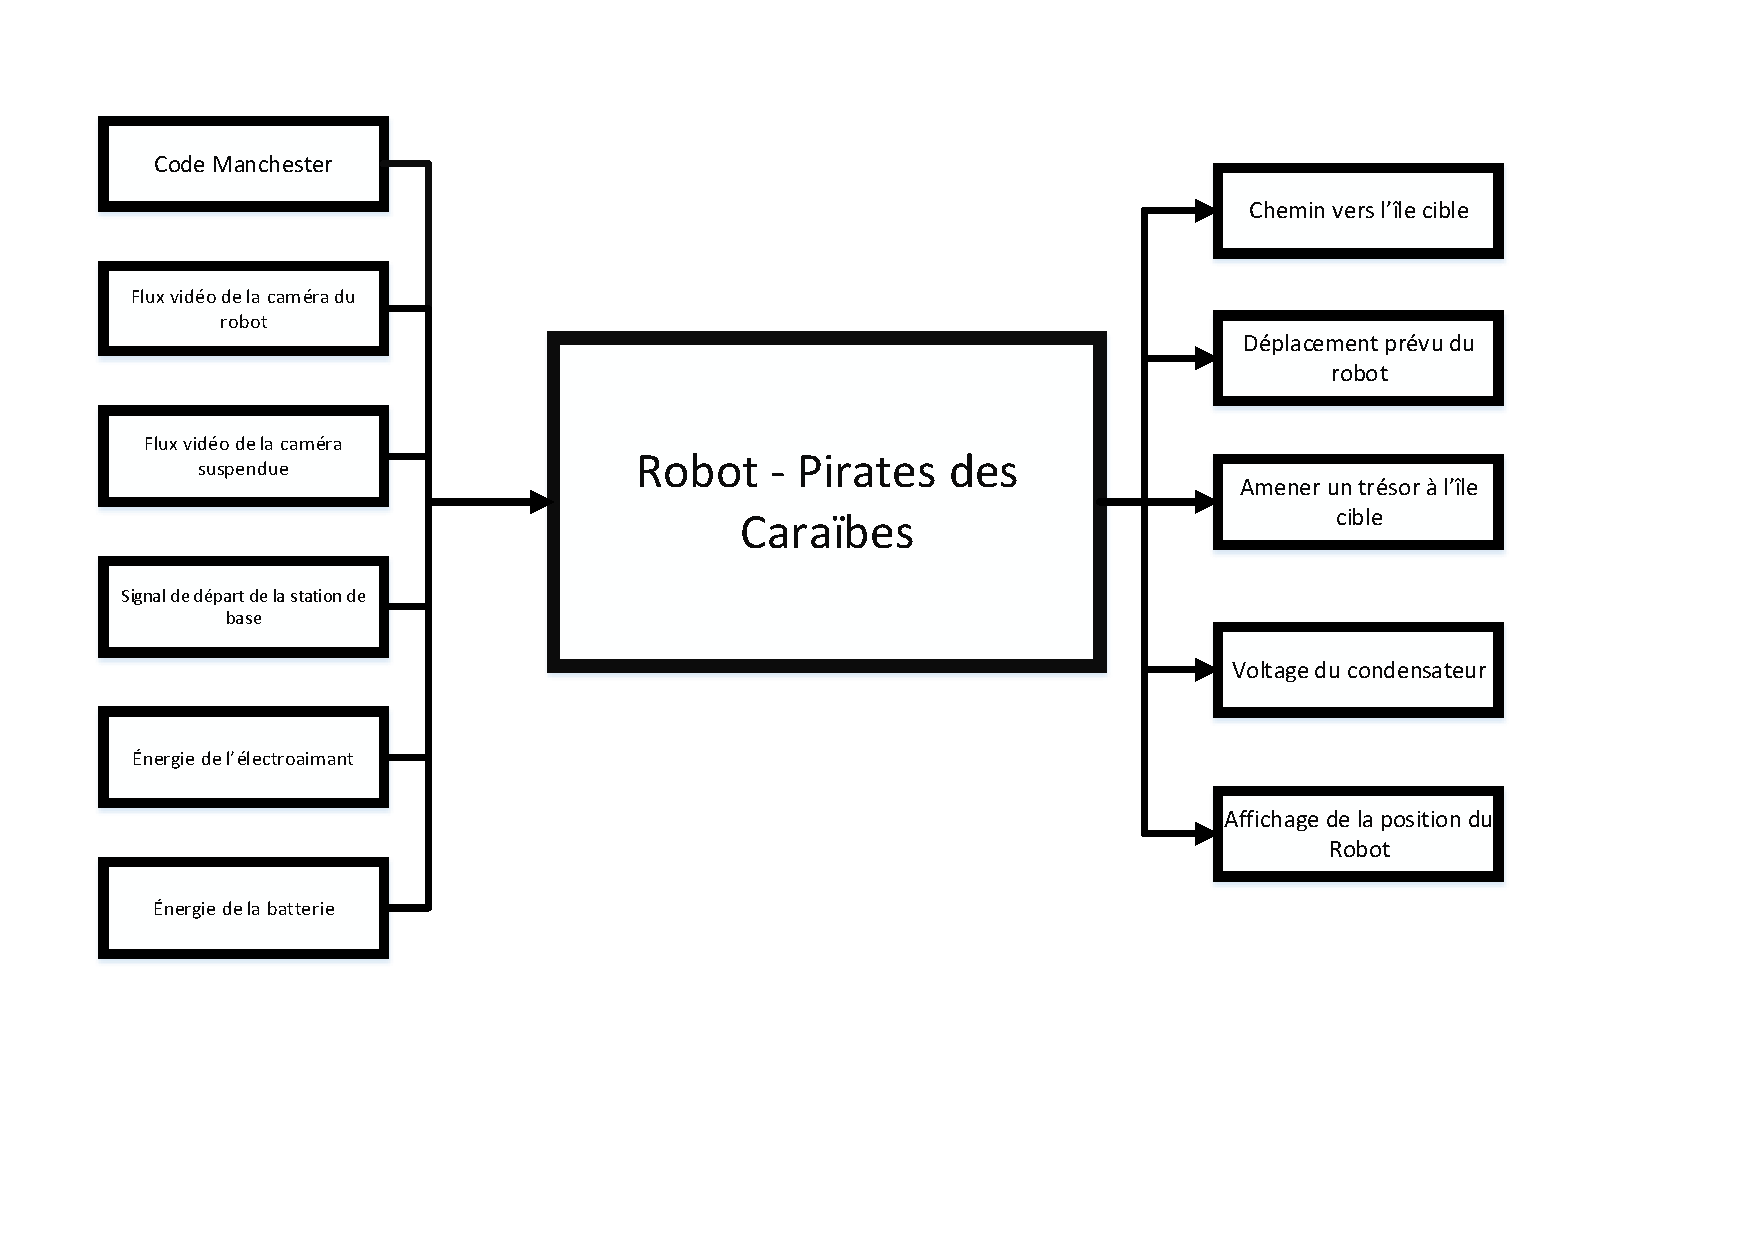
\includegraphics[scale=0.6, trim = 5mm 15mm 10mm 5mm, clip]{resources/diag_cont.pdf}
  \caption{DPF}
\end{figure}

\chapter{Diagramme des fonctionnalités}

Le diagramme des fonctionnalités permet de mettre en perspective les fonctionnalités du projet entre elles. Les fonctionnalités, les intrants et les extrants du produit y sont représentés,
ainsi que leurs relations. En effet, certaines fonctionnalités sont reliés entre elles, et certaines sont reliées aux entrées et aux sorties du système.

\begin{figure}[h]
  \centering
  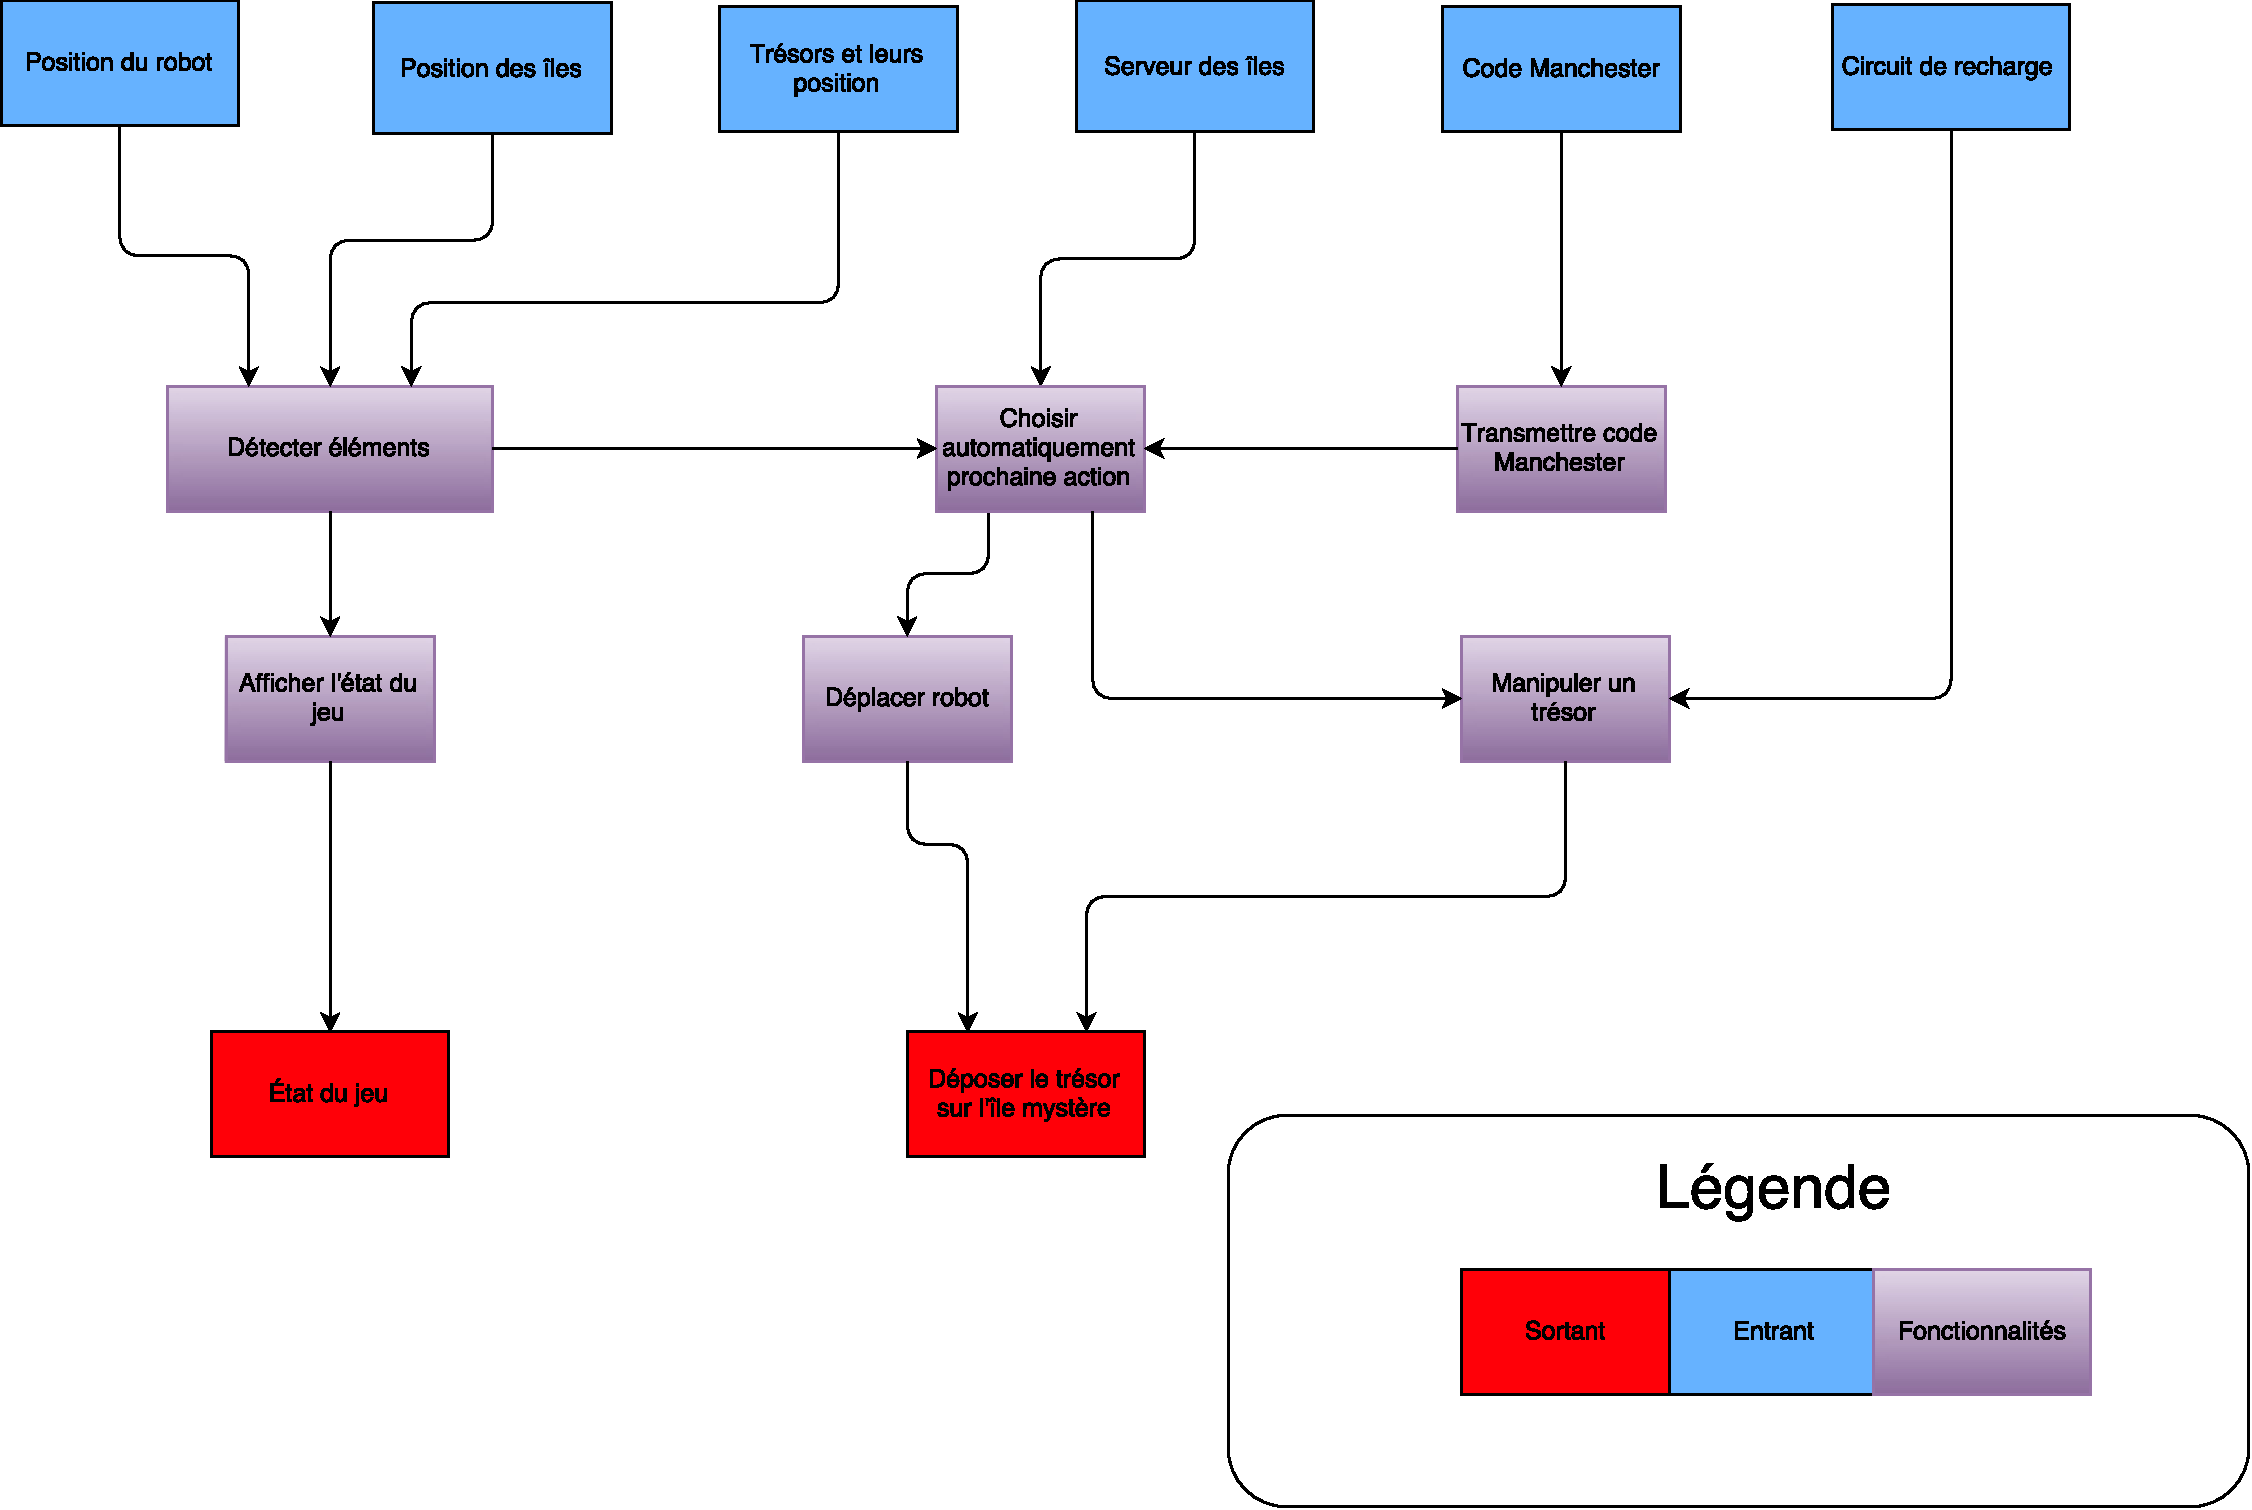
\includegraphics[scale=0.4]{resources/diag_fonc.pdf}
  \caption{Diagramme fonctionnel}
\end{figure}

\chapter{Diagramme des propriétés fonctionelles}

\begin{landscape}
\begin{figure}[h]
  \centering
  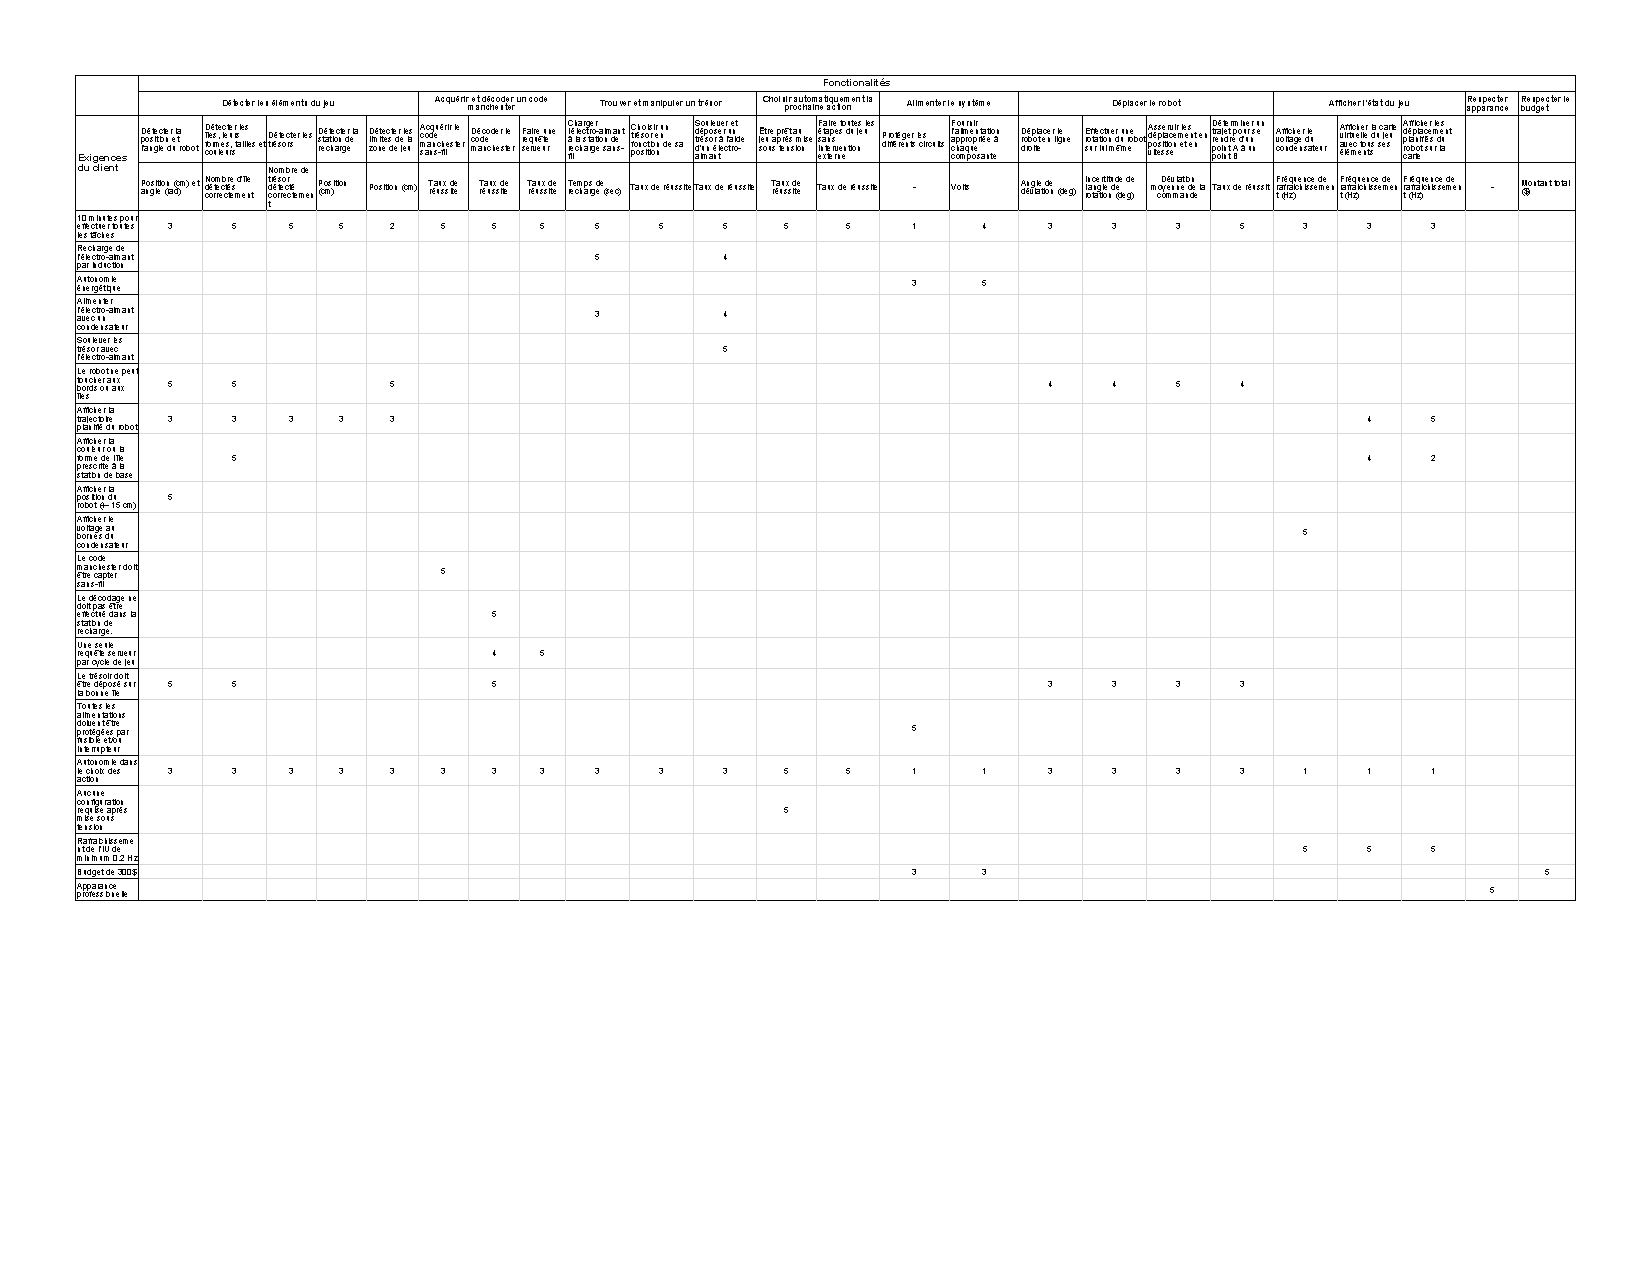
\includegraphics[scale=0.85]{resources/dpf.pdf}
  \caption{DPF}
\end{figure}
\end{landscape}

\chapter{Diagramme physique}

Les différentes fonctionnalités du projet sont implémentées par des modules physiques. Le diagramme physique permet de visualiser les fonctions accomplies par les différent modules physiques ainsi que leurs interrelations. Il permet aussi de relier les entrées et les sorties du système aux sous-systèmes physiques.

\begin{landscape}
\begin{figure}
  \centering
  \includegraphics[scale=0.5, angle=0]{resources/diagrams/physical.png}
  \caption{Diagramme physique}
\end{figure}
\end{landscape}


\chapter{Plan de test}

Les tests sont essentiels au bon fonctionnement du produit final. Ils permettent de s'assurer que le système est fonctionnel, respecte les exigences et ne contient pas de surprises. Planifier les tests permet d'accélérer et de structurer cette étape laborieuse du projet, en identifiant les objectifs et les priorités des différents tests. Chaque fonctionnalité doit être testé et documenté correctement. Le plan de tests permet donc de mettre en évidence les tests à effectuer pour chaque fonctionnalité et sous-fonctionnalités, en identifiant les paramètres à tester, la méthodologie a suivre et les équipements nécéssaires.

\begin{figure}
  \centering
  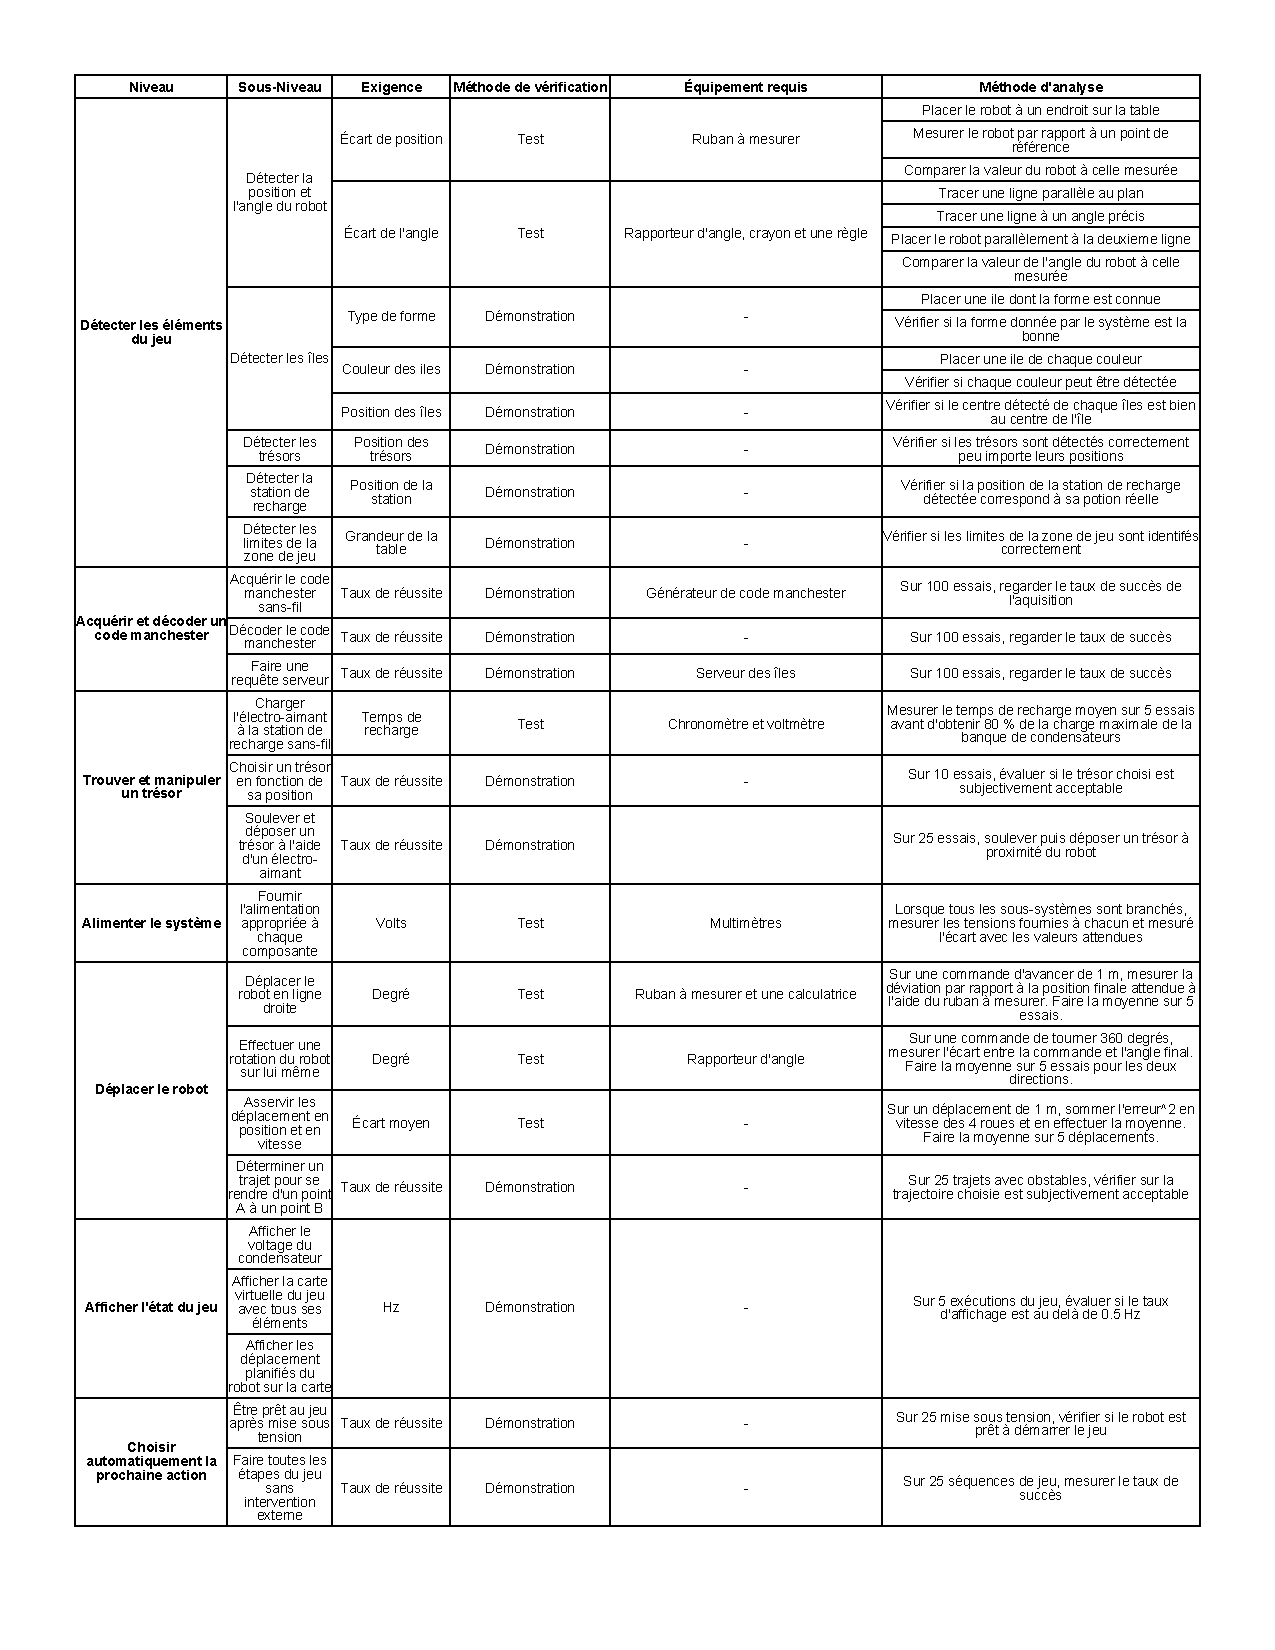
\includegraphics[scale=0.75, angle=0]{resources/tests.pdf}
  \caption{Plan de test}
\end{figure}


\chapter{Plan d'intégration}

\begin{landscape}
\begin{figure}
  \centering
  \includegraphics[scale=0.5, angle=0]{resources/diagrams/integration.png}
  \caption{Plan d'intégration}
\end{figure}
\end{landscape}


%% !TEX encoding = IsoLatin

\chapter{Cas d'utilisation}

\renewcommand{\labelitemi}{$\bullet$}
\renewcommand{\labelitemii}{$\circ$}

\section{Le robot veut se charger � la station de recharge}
\begin{description}
\item[Nom]  \hfill \\
  Recharge
\item[Acteurs] \hfill \\
  Principal : Le robot
\item[�v�nements d�clencheurs] \hfill \\
  D�part d'une s�quence
\item[Parties prenantes] \hfill \\
  Les �tudiants : Int�r�t envers la compl�tion de
  la t�che
\item[Pr�-conditions] \hfill \\
  Le condensateur est d�charg�
\item[Post-conditions] \hfill \\
  Le condensateur est charg�
\item[Sc�nario nominal] \hfill 
  \begin{itemize}
  \item D�terminer la position de la station de recharge
  \item D�terminer le chemin pour se rendre � la station de recharge
  \item Se d�placer vers la station de recharge
  \item Se recharger
  \end{itemize}
\item[Contraintes] \hfill
  \begin{itemize}
  \item Doit �viter les �les lors des d�placements
  \end{itemize}
\end{description}

\section{Le robot veut conna�tre l'�le de destination.}
\begin{description}
\item[Nom] \hfill \\
  Transmission de la cible  
\item[Acteurs] \hfill \\
  Principal : Le robot \\
  La station de recharge \\
  Le serveur d'�les
\item[�v�nements d�clencheurs] \hfill \\
  Le robot se situe � la station de recharge
\item[Parties prenantes] \hfill \\
  Les �tudiants : Int�r�t envers la compl�tion de la t�che \\
  Station de recharge : Transmettre son message
\item[Pr�-conditions] \hfill \\
  Le robot se situe � la station de recharge
\item[Post-conditions] \hfill \\
  Le robot conna�t les informations de l'�le cible
\item[Sc�nario nominal] \hfill
  \begin{itemize}
  \item Obtenir la lettre en code Manchester
  \item R�cup�rer les caract�ristiques de l'�le aupr�s du serveur des �les 
  \item Associer la lettre � l'�le de destination
  \end{itemize}
\end{description}

\section{Le robot veut aller chercher un tr�sor}
\begin{description}
\item[Nom] \hfill \\
  R�cup�ration du tr�sor
\item[Acteurs] \hfill \\
  Princpal : Le robot
\item[�v�nements d�clencheurs] \hfill \\
  Le robot conna�t sa destination et la recharge est termin�e
\item[Parties prenantes] \hfill \\
  Les �tudiants : Int�r�t envers la compl�tion de la t�che \\
  Le robot : Int�r�t � obtenir le tr�sor
\item[Pr�-conditions] \hfill \\
  Le robot conna�t les informations sur l'�le de destination
\item[Post-conditions] \hfill \\
  Le robot a pris possession du tr�sor optimal selon la position de l'�le
\item[Sc�nario nominal] \hfill
  \begin{itemize}
  \item Selon l'�le de destination, d�terminer le tr�sor ayant la position
    optimale ainsi que le chemin pour s'y rendre
  \item Se d�placer vers le tr�sor choisi
  \item Prendre possession du tr�sor
  \end{itemize}
\item[Contraintes] \hfill \\
  Doit �viter les �les lors des d�placements
\end{description}

\section{Le robot veut d�poser le tr�sor sur l'�le de destination}
\begin{description}
\item[Nom] \hfill \\
  D�p�t du tr�sor
\item[Acteurs] \hfill \\
  Principal : Le robot
\item[�v�nements d�clencheurs] \hfill \\
  Le robot a pris posession du tr�sor
\item[Parties prenantes] \hfill \\
  Les �tudiants : Int�r�t envers la compl�tion de la t�che \\
  Le robot : Int�r�t � d�poser le tr�sor au bon endroit
\item[Pr�-conditions] \hfill \\
  Le robot conna�t les informations sur l'�le de destination et le robot est en posession du tr�sor
\item[Post-conditions] \hfill \\
  Le tr�sor est d�pos� sur l'�le
\item[Sc�nario nominal] \hfill
  \begin{itemize}
  \item D�terminer le chemin optimal pour se rendre � l'�le de destination
  \item Se rendre � l'�le
  \item D�poser le tr�sor sur l'�le de destination
  \end{itemize}
\item[Contraintes] \hfill
  \begin{itemize}
  \item Doit �viter les �les lors des d�placements
  \item Doit se rendre jusqu'� l'�le avant que l'aime ne se d�charge
  \item Le tr�sor doit toucher � l'�le
  \end{itemize}
\end{description}

\chapter{Diagrammes Logiciel}
Les prochains diagrammes ont pour but de présenter l'idée de départ de notre architecture logicielle.
En effet, bien que ceci constitue notre architecture visée, cette dernière changera inéluctablement lors du développement, comme le veut la gestion de projet "Agile".
Autre précision, ces diagrammes modélisent seulement les tranches les plus utiles afin d'avoir une bonne vision de l'ensemble du système.

\begin{landscape}
\begin{figure}
  \centering
  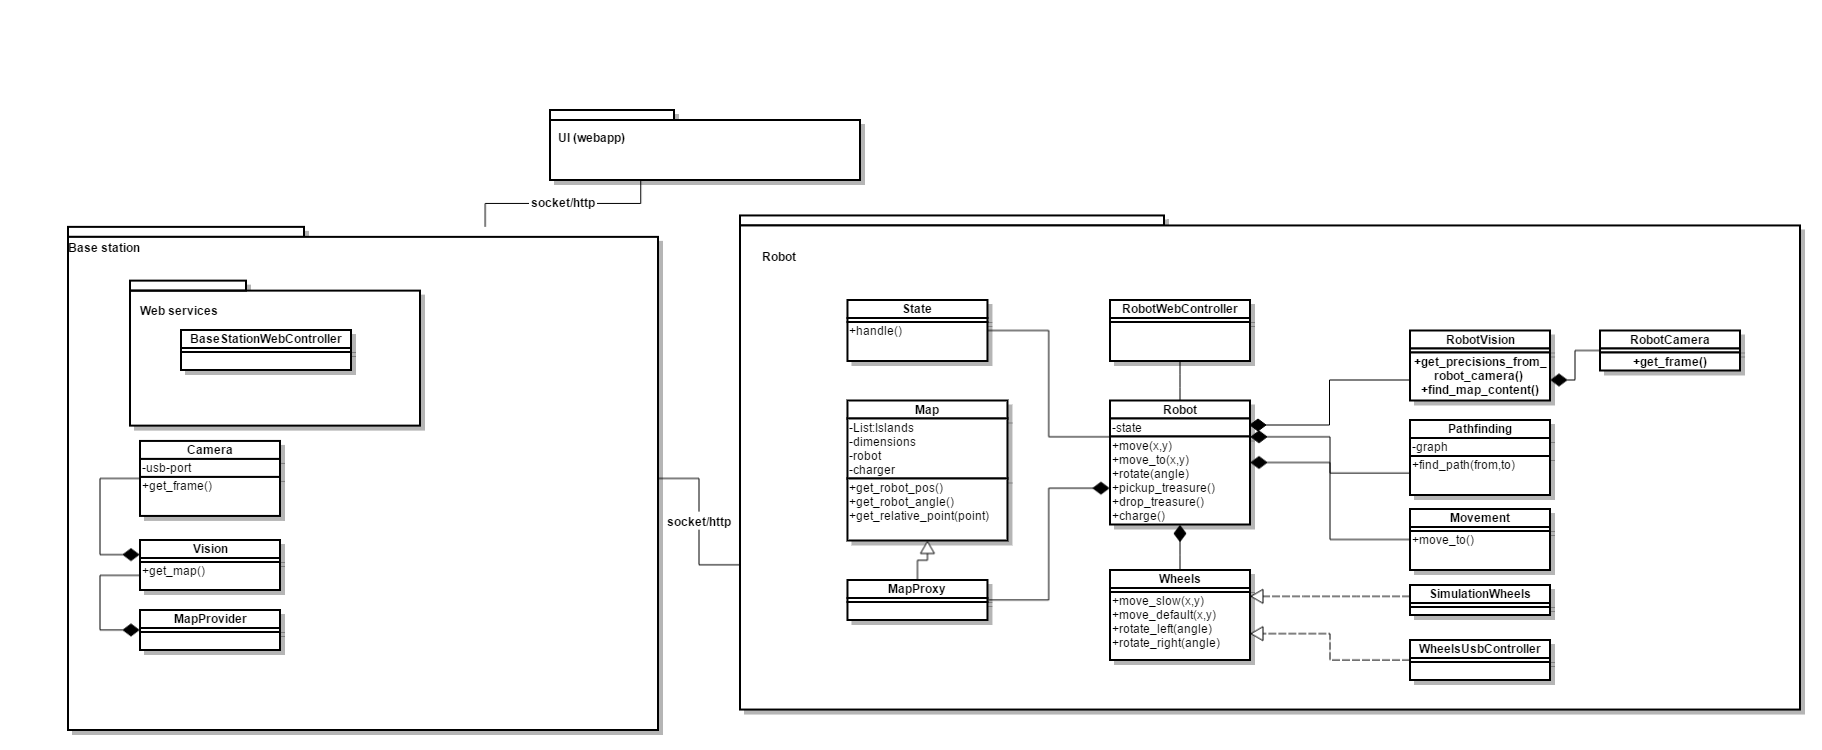
\includegraphics[scale=0.4, angle=0]{resources/diagrams/classDiagram.png}
  \caption{Diagramme de classe}
\end{figure}

\begin{figure}
  \centering
  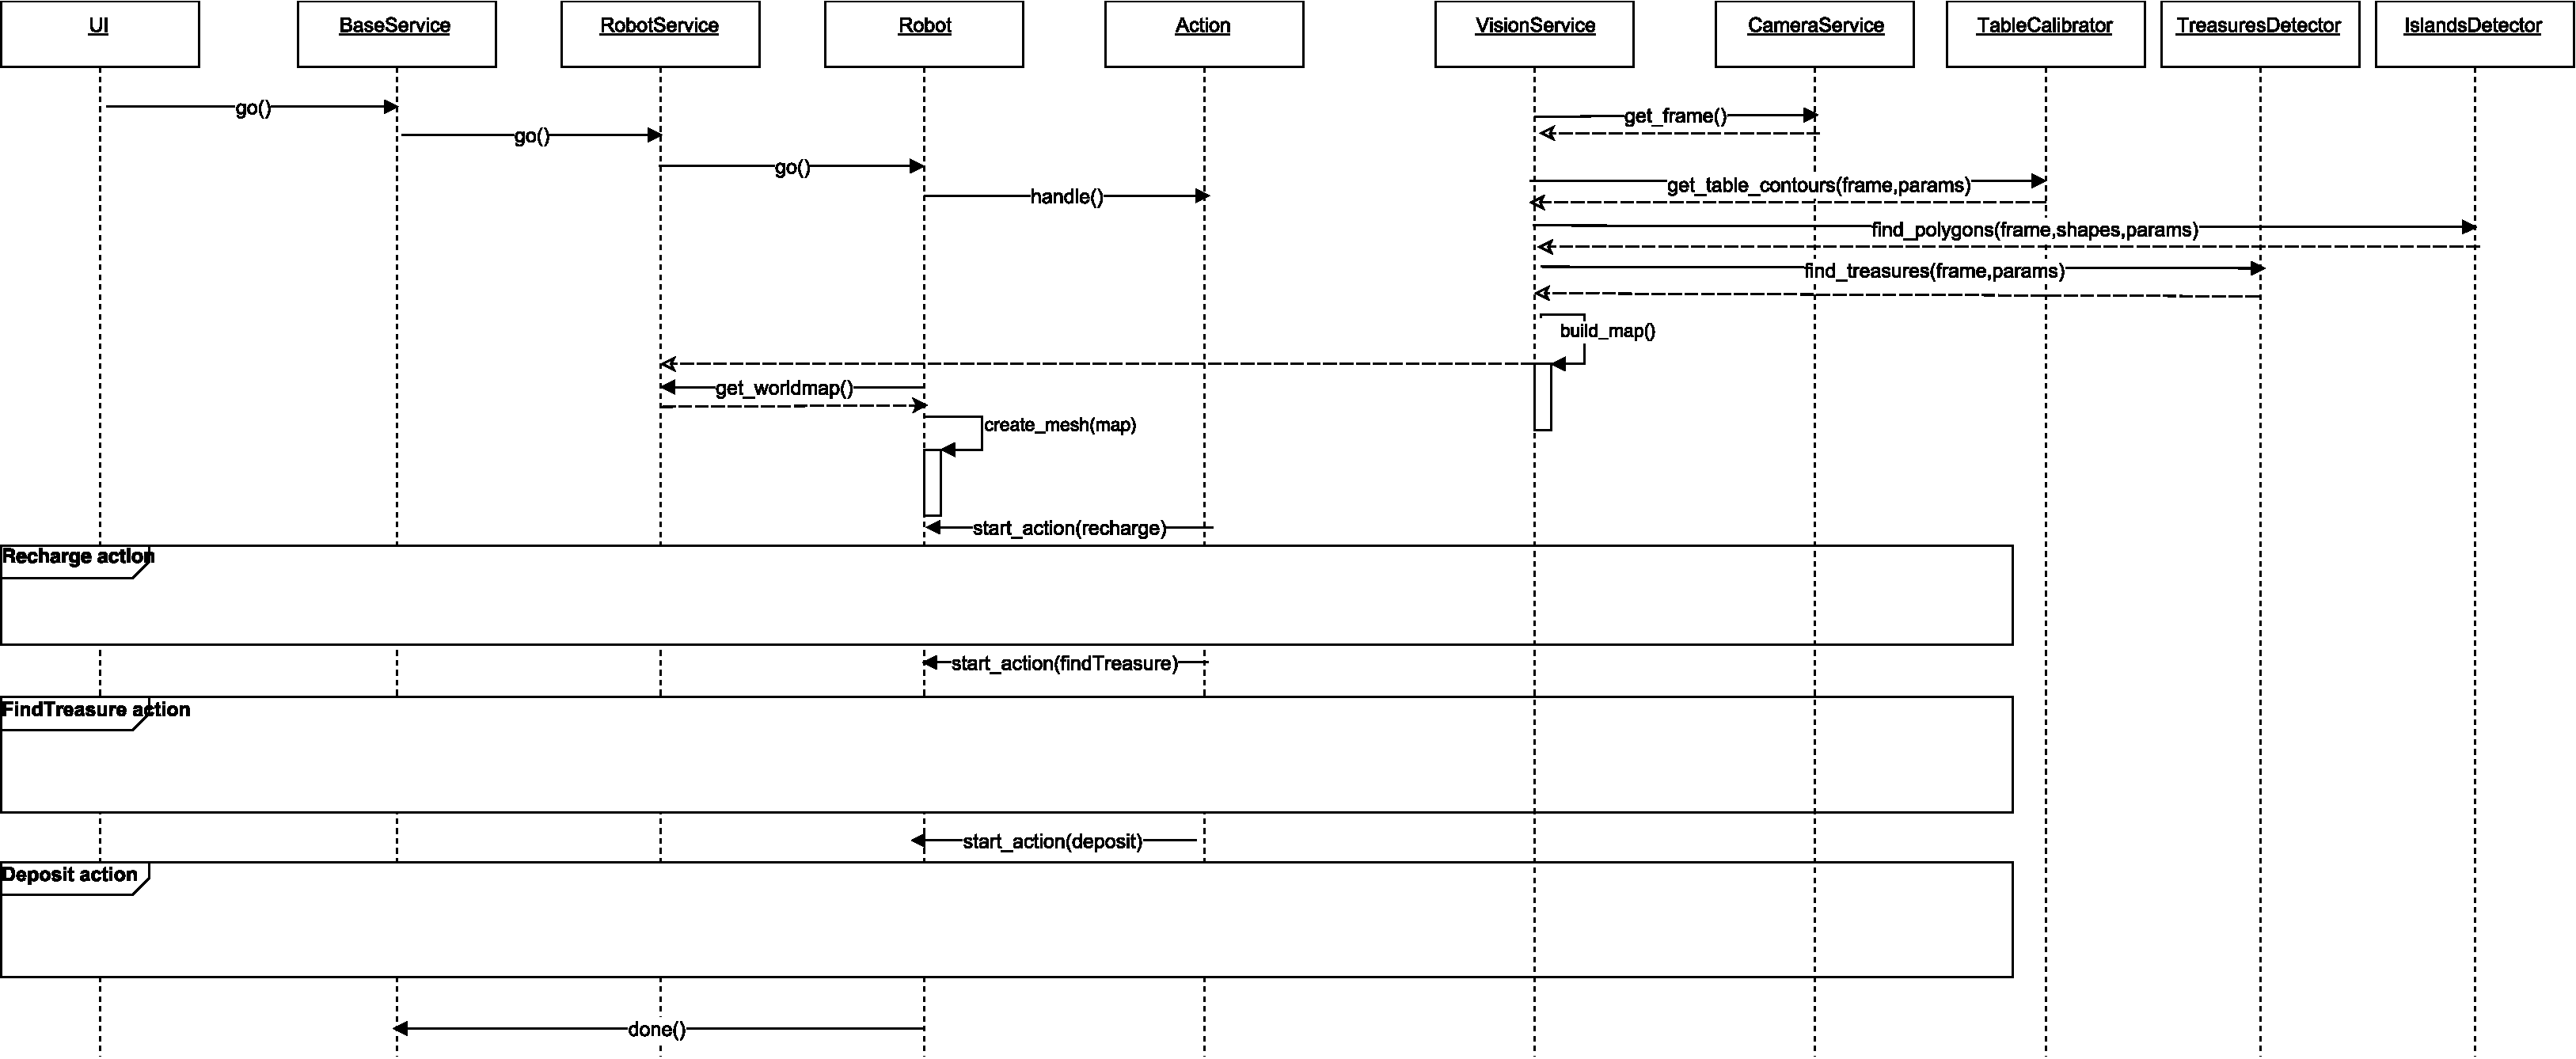
\includegraphics[scale=0.45, angle=0]{resources/diagrams/sequenceDiagram.pdf}
  \caption{Diagramme de séquence complet}
\end{figure}

\begin{figure}
  \centering
  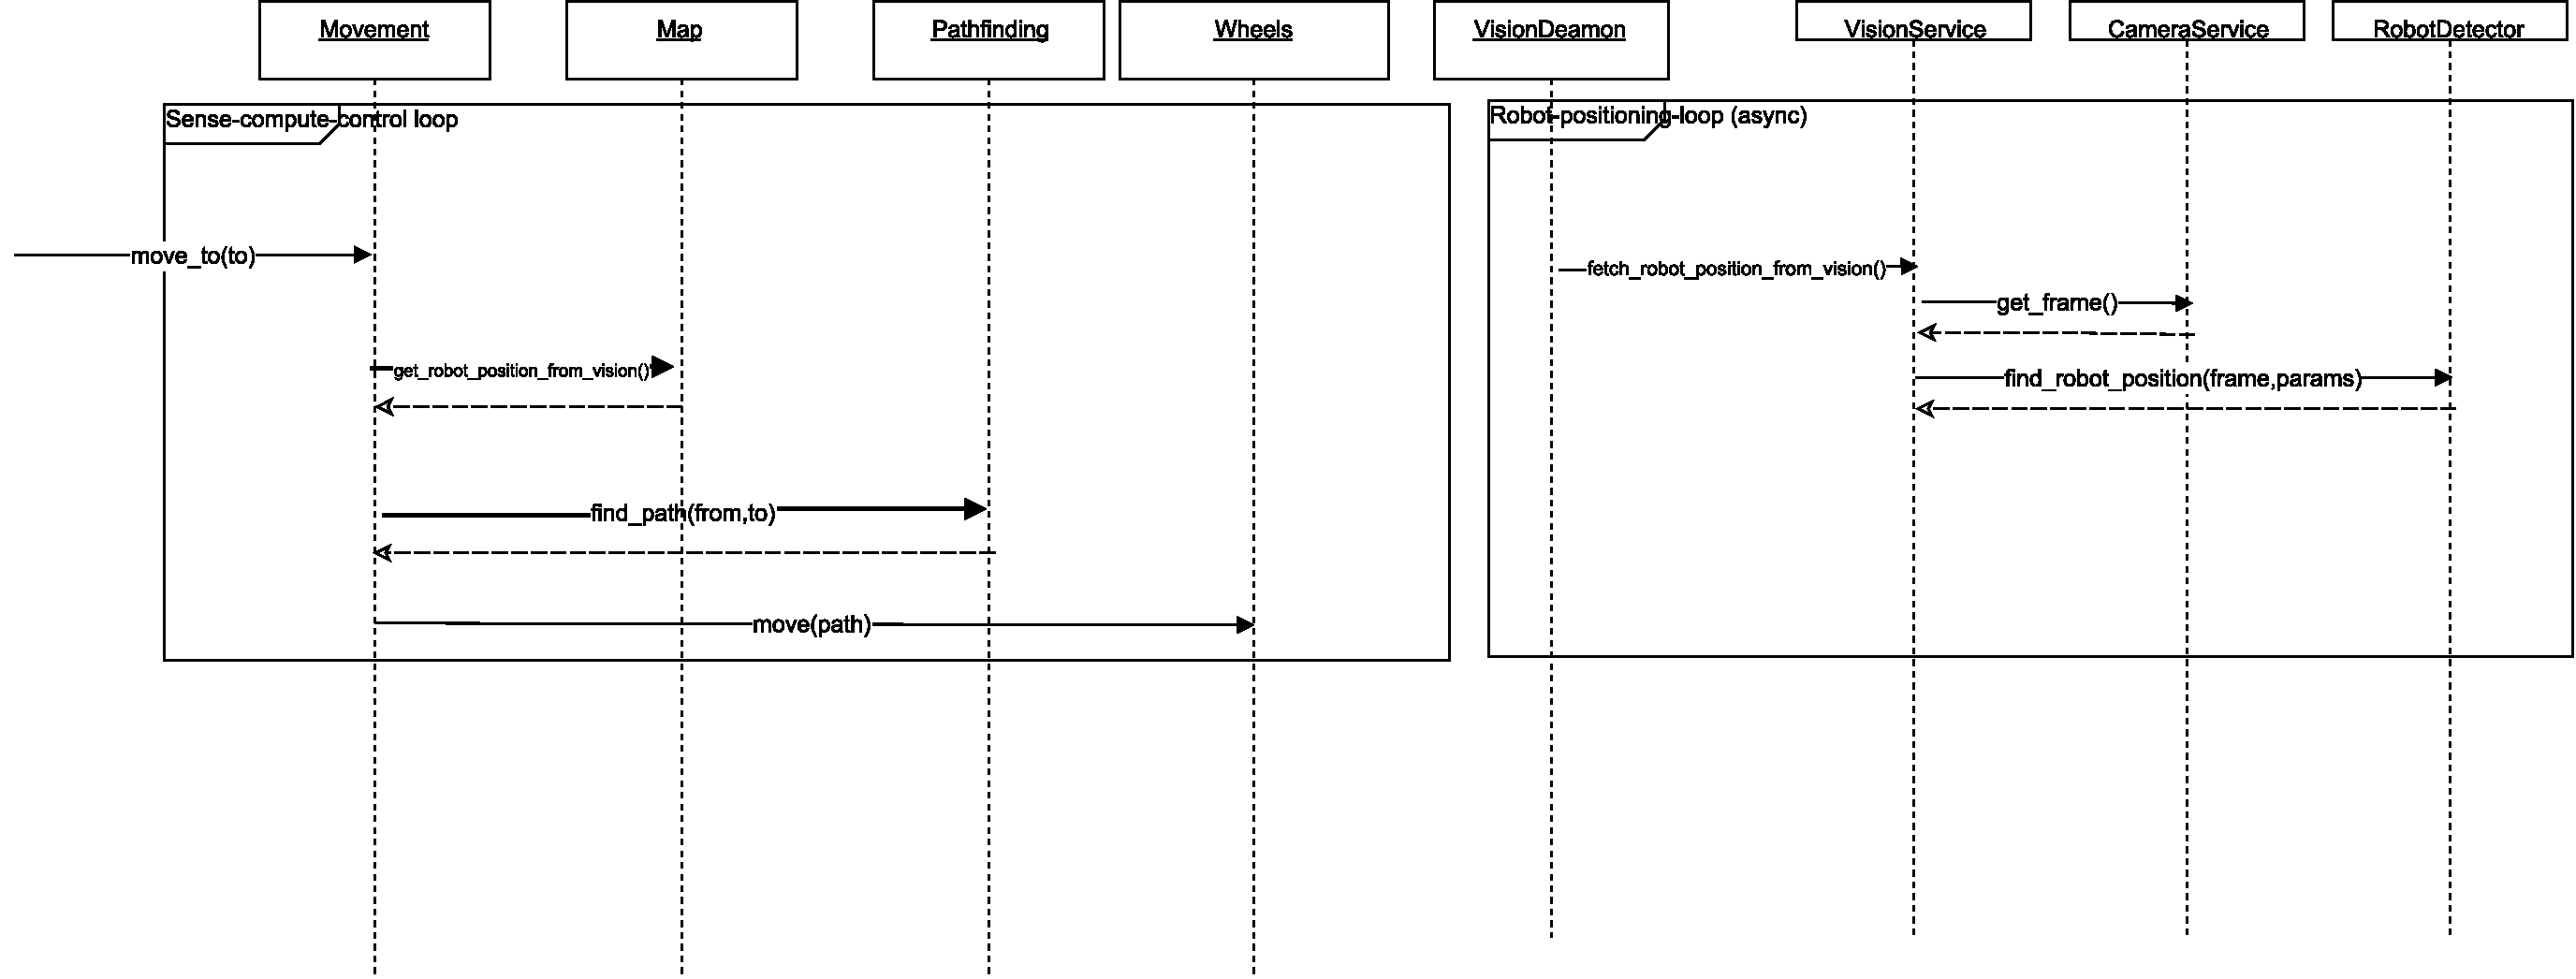
\includegraphics[scale=0.45, angle=0]{resources/diagrams/robotMovement.pdf}
  \caption{Diagramme de séquence de la boucle de sense-compute-control lors d'un déplacement}
\end{figure}

\begin{figure}
  \centering
  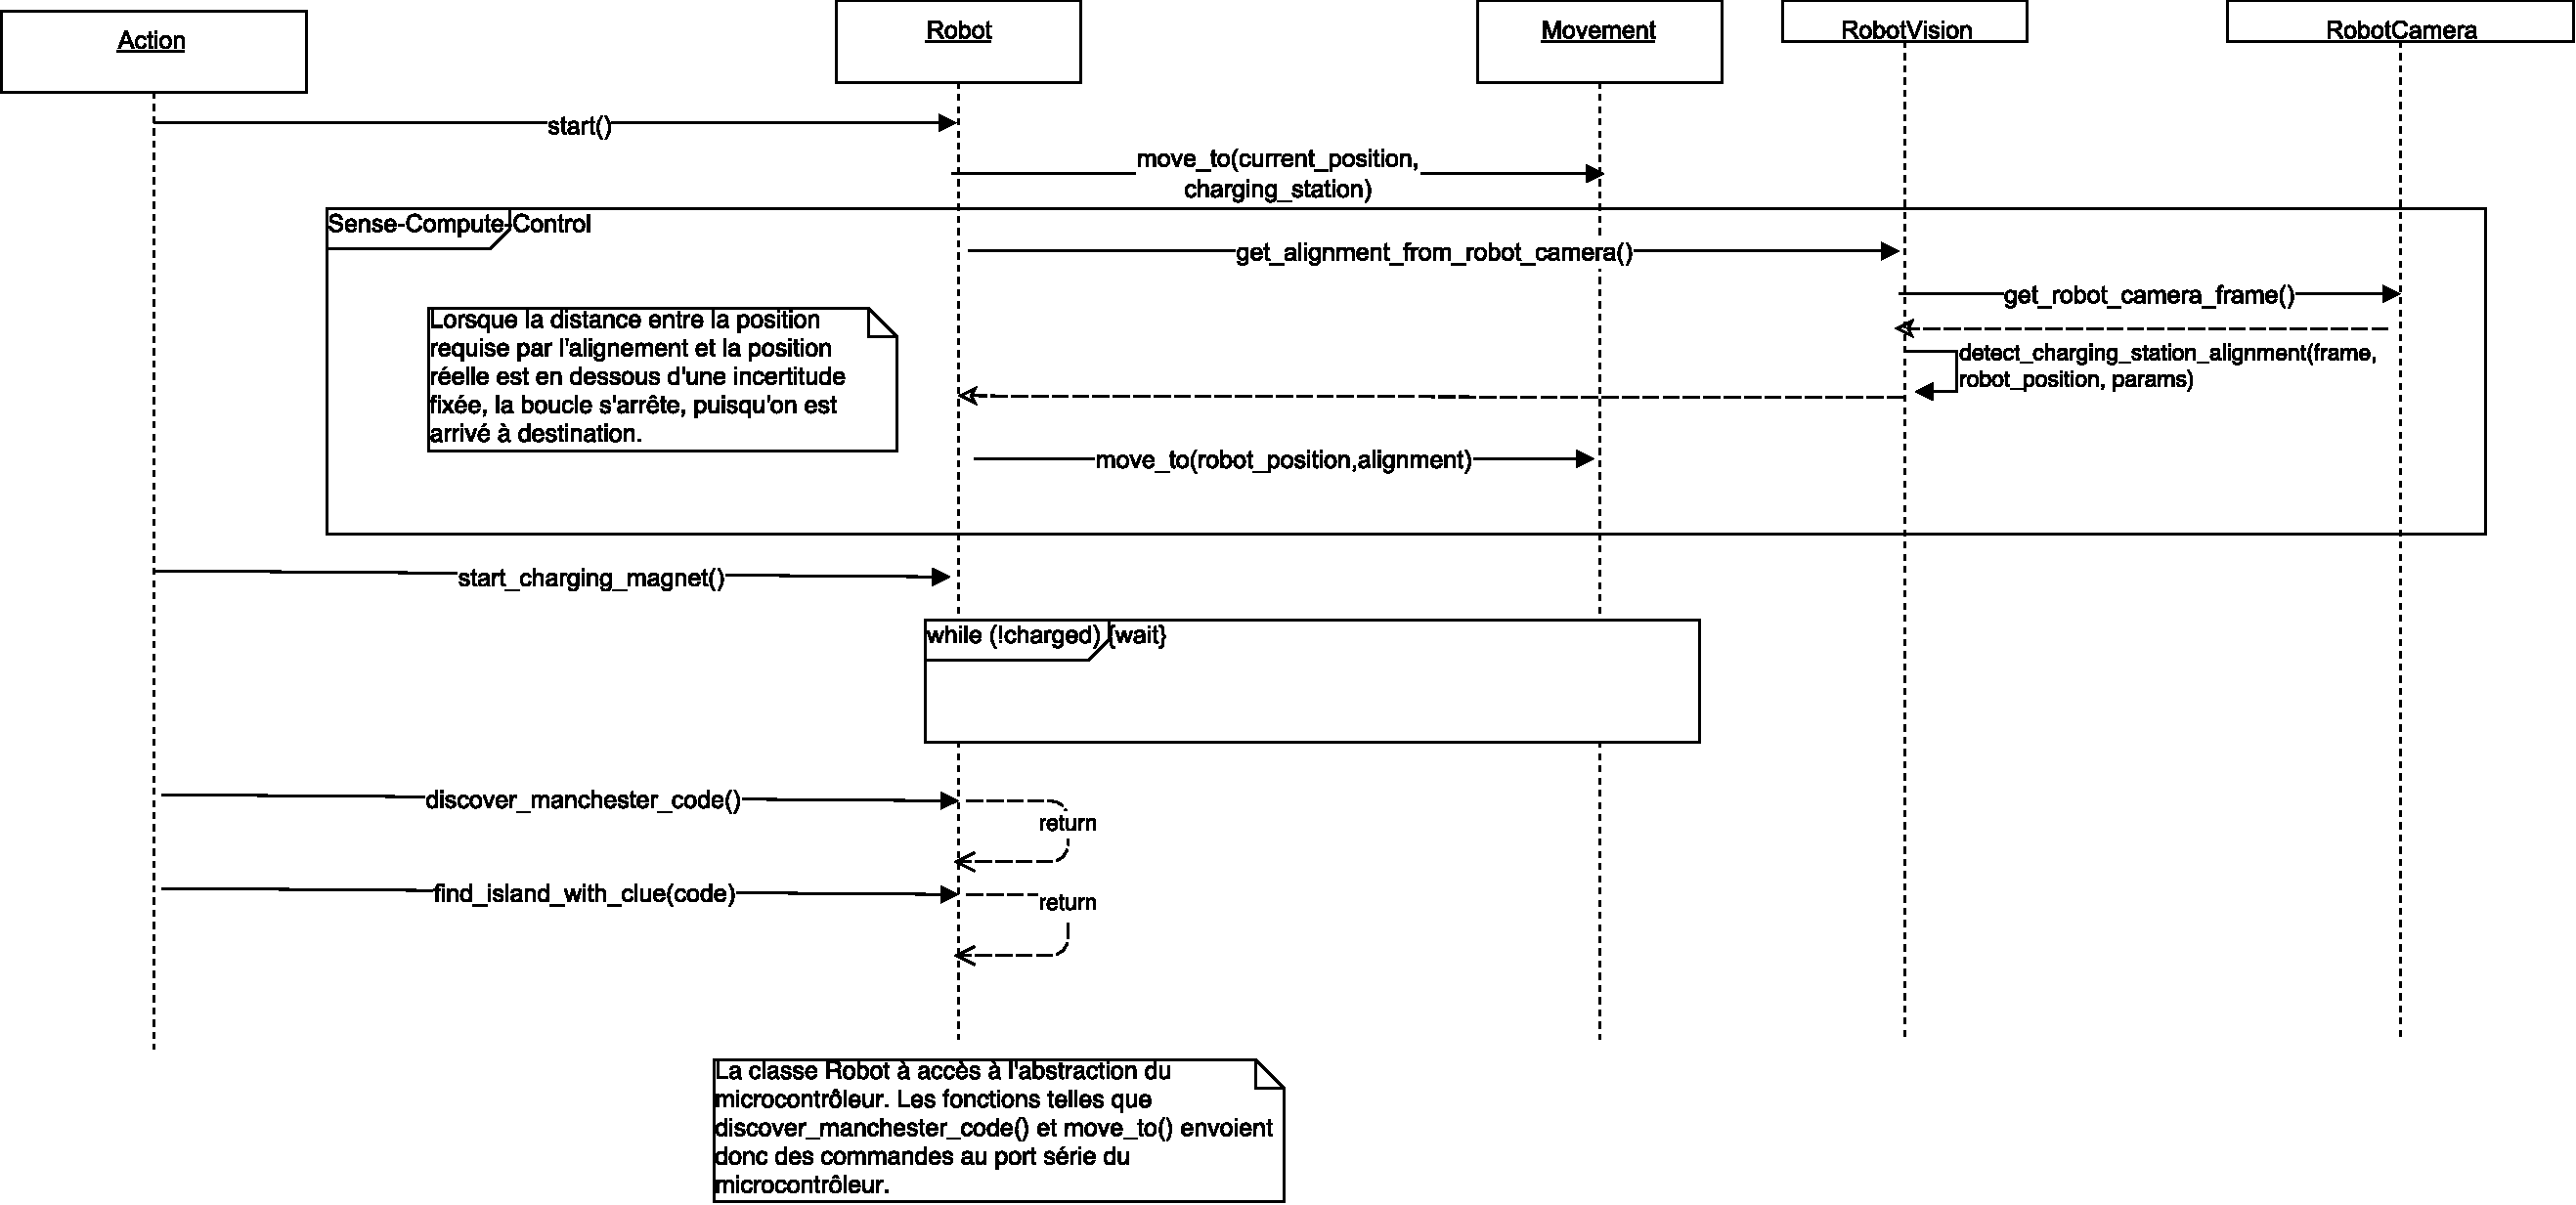
\includegraphics[scale=0.5, angle=0]{resources/diagrams/rechargeAction.pdf}
  \caption{Diagramme de séquence de recharge}
\end{figure}

\begin{figure}
  \centering
  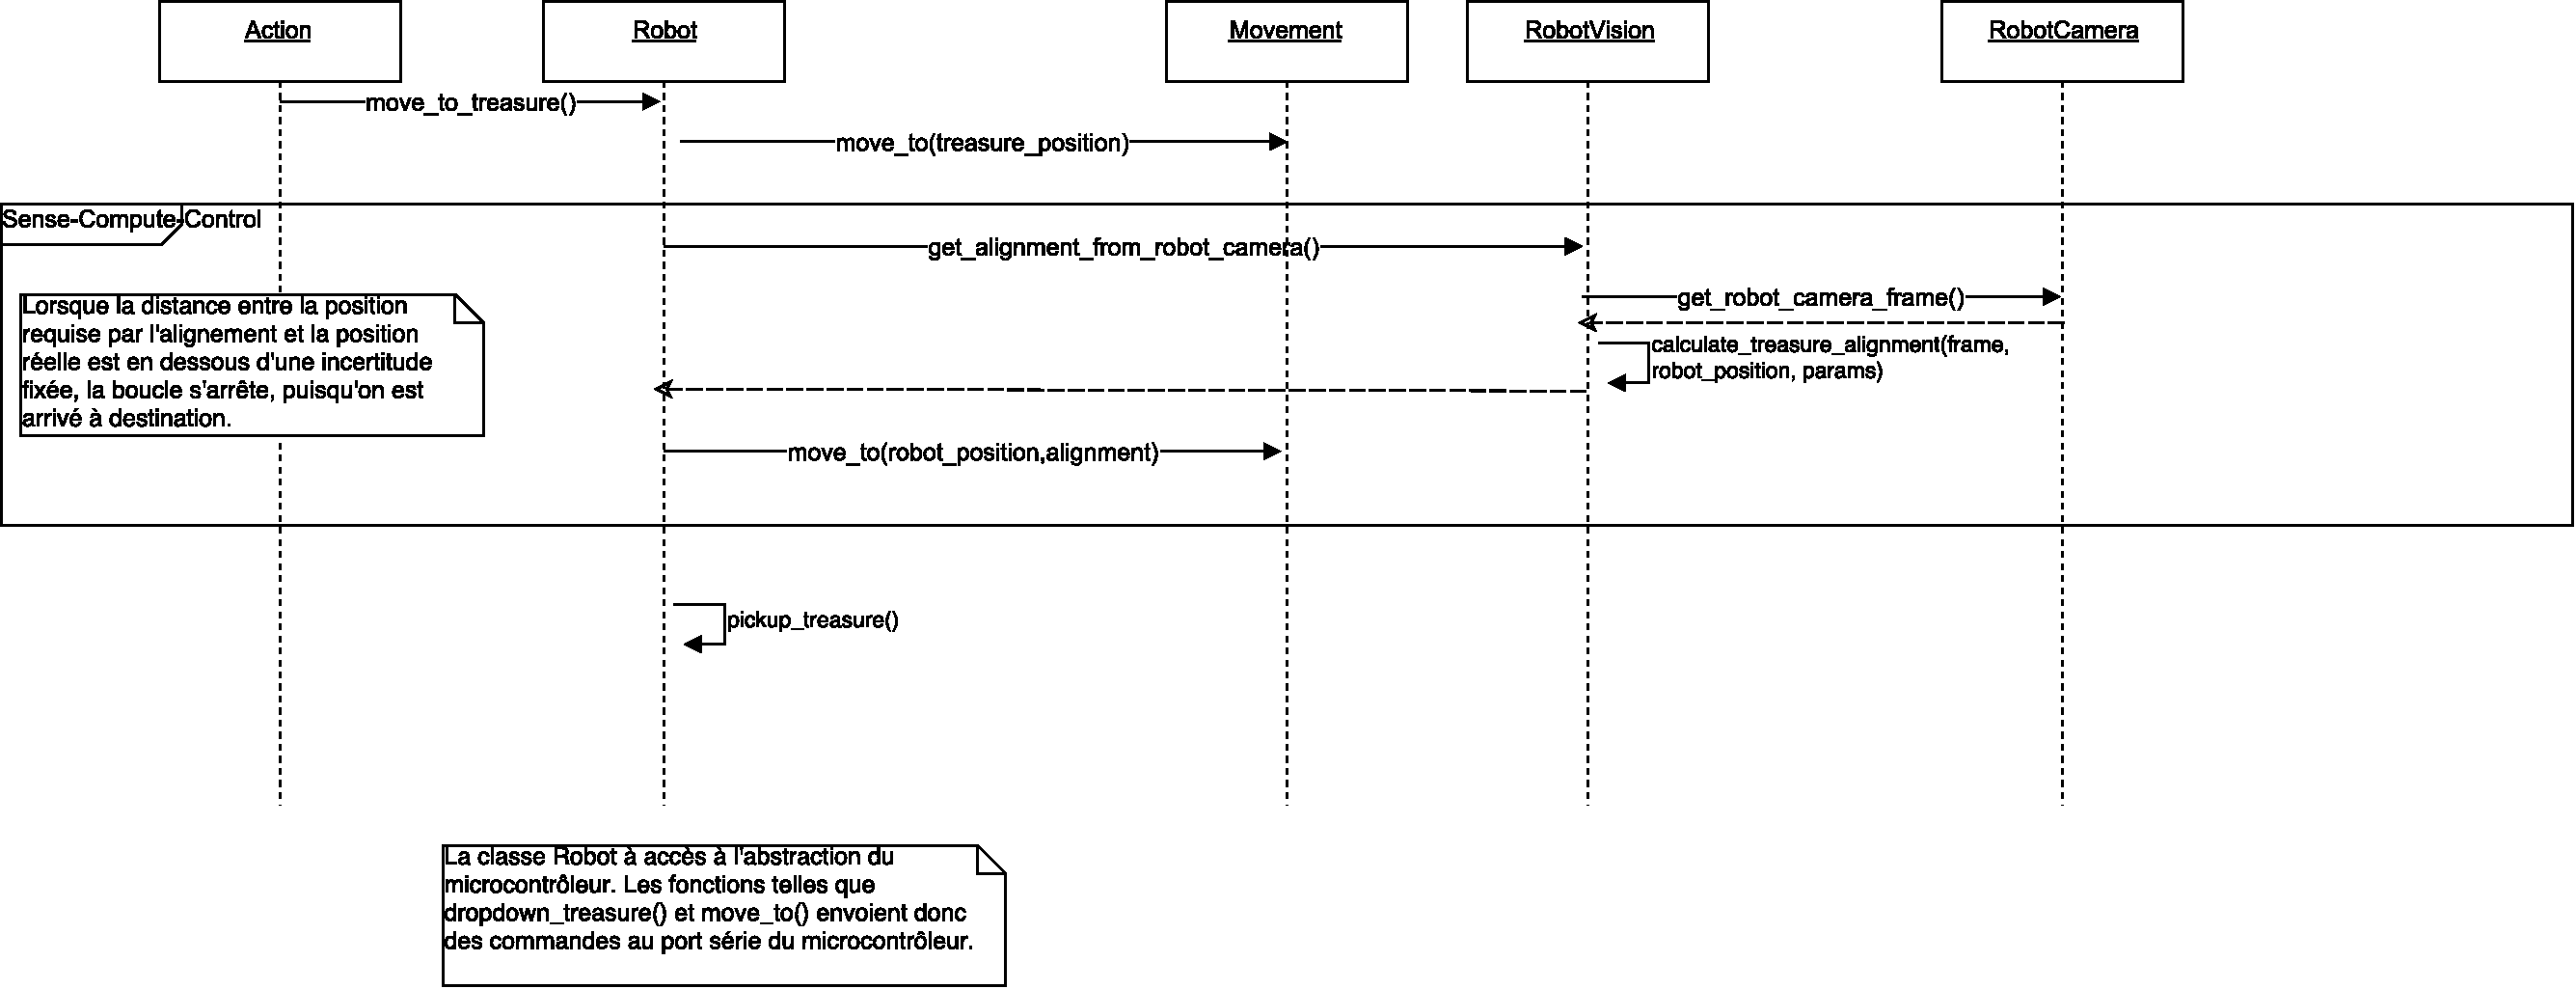
\includegraphics[scale=0.4, angle=0]{resources/diagrams/findTreasureAction.pdf}
  \caption{Diagramme de séquence de recherche de trésor}
\end{figure}

\begin{figure}
  \centering
  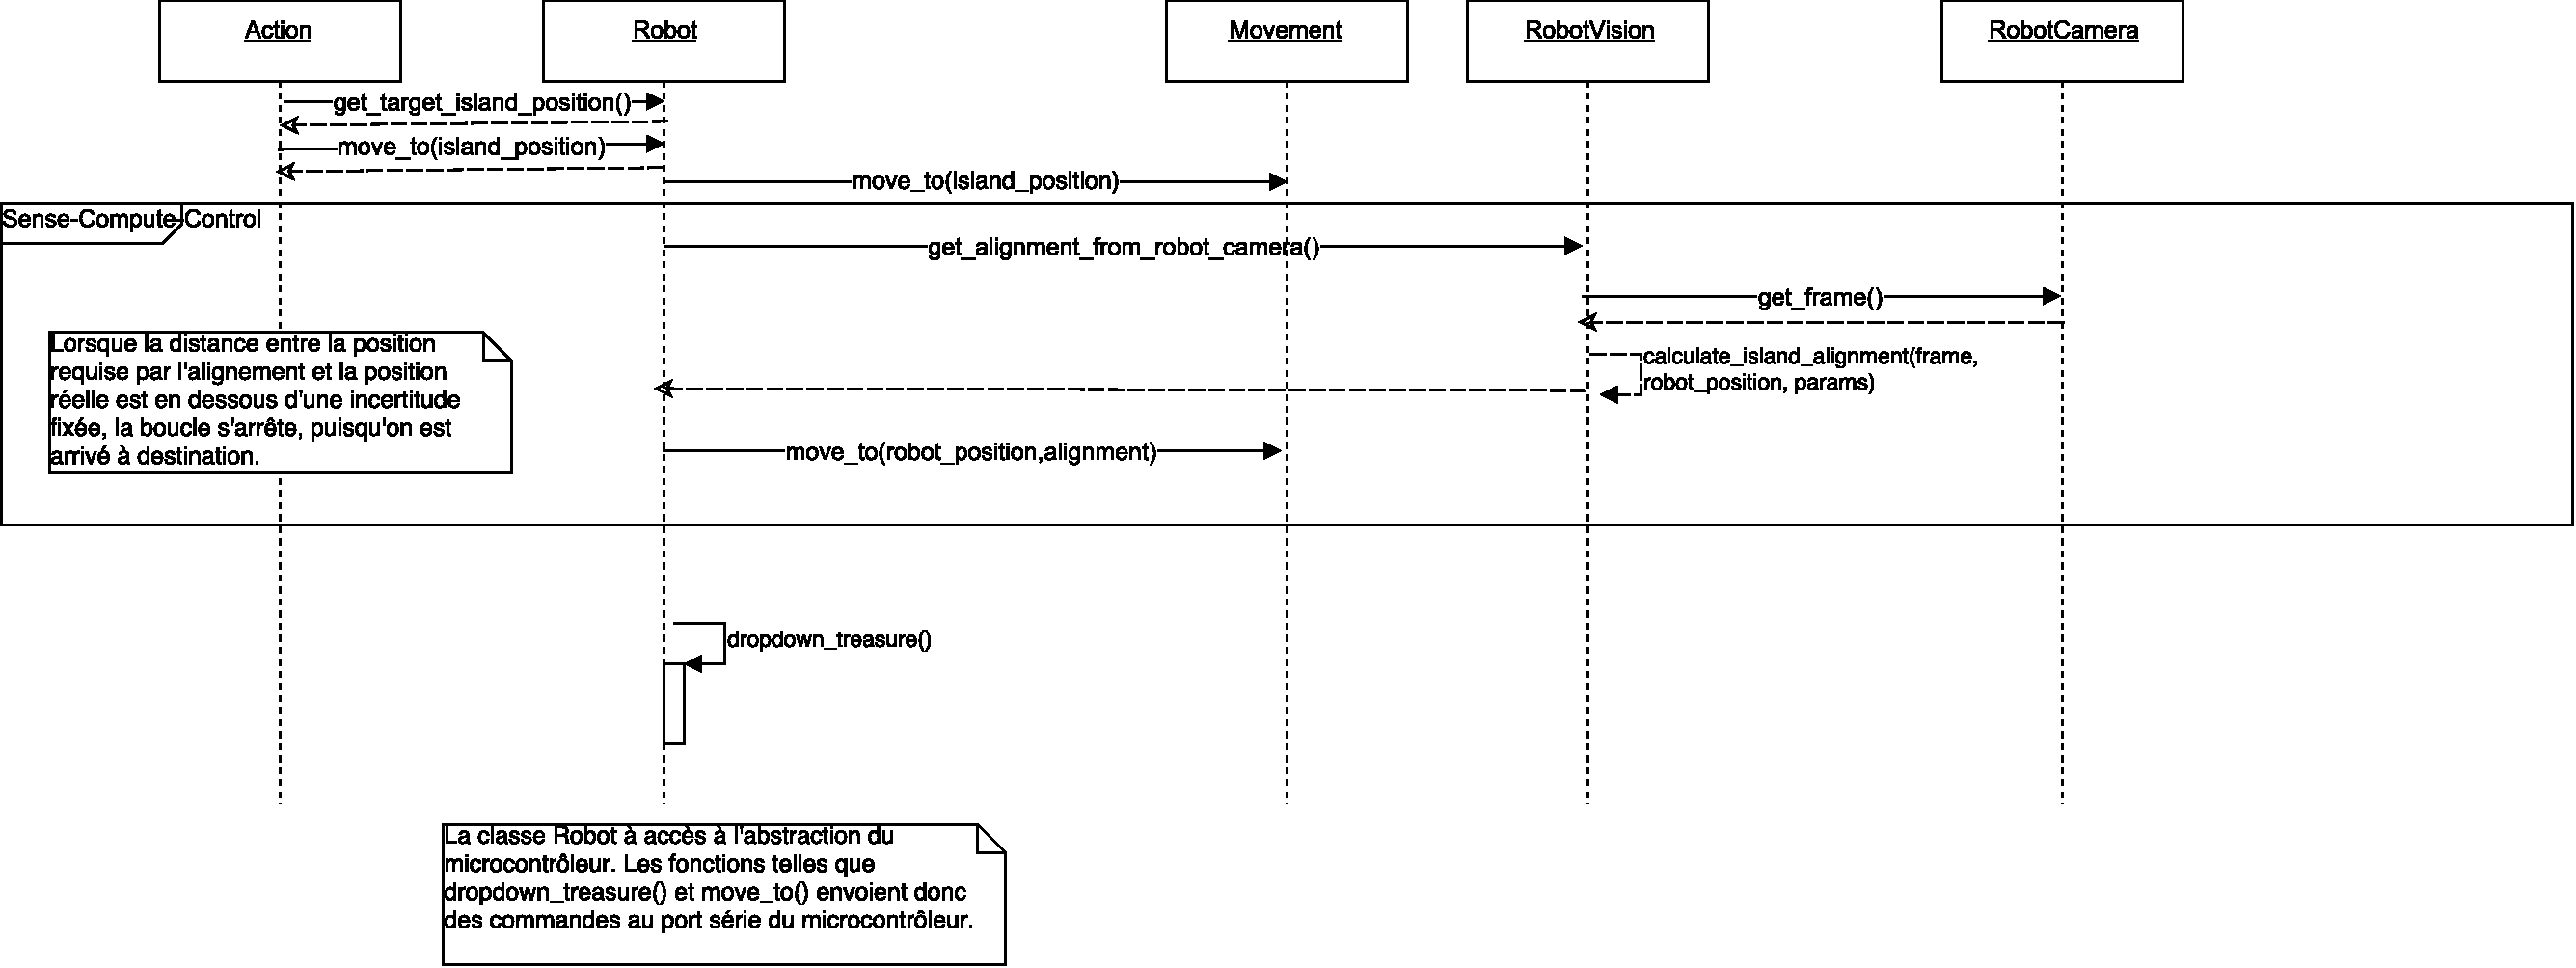
\includegraphics[scale=0.5, angle=0]{resources/diagrams/depositAction.pdf}
  \caption{Diagramme de séquence dépot du trésor}
\end{figure}
\end{landscape}

\chapter{Tests unitaires}

Voir le code source.
Les test peuvent être exécutés à l'aide de nosetests.
Pour le coverage, utiliser la commande "nosetests --with-coverage"

%%!TEX encoding = IsoLatin
\chapter{Exp�riences pr�liminaires}

\section{Arduino Mega}

Comme microcontr�leur, nous avons d�cid� d'utilise le Arduino Mega. En plus d'offrir un I/O assez g�n�reux, la facilit� d'utilisation et l'�norme communaut� Arduino en ligne en font une solution accessible et permettant de d�ployer rapidement de nouvelles fonctionnalit�s � partir des nombreuses librairies disponibles en ligne. Un pinout pr�liminaire fut �tabli afin de confirmer si la quantit� de broches et de p�riph�rique �tait suffisante.

\section{Pont en H et commande de moteur}

Afin de tester les moteurs, nous avons commenc� � interfacer un canal de pont en H avec un moteur et le Arduino. Nous avons donc alimenter le circuit avec une source DC 12 V limit�e en courant � 1.5 A. Cette limite fut d�cid� arbitrairement afin d'�viter de mauvaises surprises. Le moteur fut aliment� par le canal 3. Ensuite, les 3 broches de contr�le du canal 3 furent branch�es � 3 broches de sortie du Arduino. Ces broches permettent de contr�ler l'activation du moteur, sa direction et sa vitesse.  La broche de vitesse fut branch� � une sortie de type PWM 8 bits (256 valeurs). Ainsi, nous avons �valu� le seuil de d�part � vide de la roue ainsi que la consommation � la vitesse maximale. 

\section{Encodeurs}

L'encodeur sur les roues offre 2 canaux, chacun donnant 16 impulsions par tour de moteur. En comptant les fronts montants et descendants de chaque canal, l'encodeur offre 64 steps par tour de moteur. Avec une transmission 100:1, cela offre un potentiel de 6400 steps par r�volution de roue, ce qui est beaucoup, voir trop pour notre application.  Comme premier test, on a branch� le canal 1 des 4 encodeurs sur 4 broches d'interruption du Arduino Mega. La fonction ISR de chaque canal d'interruption fut configur� afin de compter le nombre de fronts montants. Pour l'instant, la quantit� d'interruption ne semble pas causer de probl�me � l'int�rieur de la boucle principale du programme, mais d'autres tests seront n�c�ssaire afin d'assurer la robustesse de ce principe d'aquisition.

\section{Asservissement en vitesse des moteurs}

Des tests pr�liminaires d'asservissement en vitesses furent effectu�s sur 2 roues comme preuve de concept. Ainsi, un intervalle dt fut �tabli � 100 ms. Apr�s ce dernier, la vitesse d�sir�e pour chaque roue est compar�e avec la vitesse actuelle. Un PID arbitraire fut appliqu� ensuite en fonction de cette erreur. Rapidement, on a trouv� des param�tres assez stables, permettant au syst�me de subir quelques perturbations et de revenir rapidement � la vitesse d�sir�e. Durant nos tests, nous avons eu des probl�mes � synchroniser deux roues ensemble. En effet, l'utilisation de la fonction AnalogWrite() dans la boucle d'asservissement sur plusieurs broches simultan�es entrainait des comportements impr�visibles. Apr�s recherche, nous avons d�cid� de coder manuellement la fonction de sortie PWM et le probl�me fut r�gl�. Par la suite, en comparant la vitesse de deux roues, un facteur suppl�mentaire fut ajout� � la boucle d'asservissement permettant de ralentir la roue qui va plus vite que l'autre et vice-versa. Ainsi, nos tests pr�liminaires d'asservissement nous ont permis de synchroniser deux roues en vitesse et en position.

\section{Observations g�n�rales}
  La base en aluminium offre un excellent support aux roues. La r�sistance de la base permet l'ajout d'�tage sup�rieur tout en conservant la solidit� structurale du robot. Les bases des �tages sup�rieurs sont l�g�res et non conductrices. Un centre de gravit� relativement bas est n�cessaire pour �liminer tout d�balancement du robot durant ses d�placements. C'est pourquoi les pi�ces les plus lourdes se situeront autant que possible sur les �tages inf�rieurs.

Les roues poss�dent un jeu de quelques degr�s en rotation. Ce degr� de libert� n'implique pas l'arbre du moteur. En cons�quence, les d�codeurs raccord�s � l'arbre ne d�tectent pas ce d�placement suppl�mentaire. Il reste � d�terminer si cette caract�ristique peut devenir probl�matique. 

\section{Communications sans fil}
  Une carte interne sans fils de 2.4Ghz � deux sorties est pr�sente sur la carte m�re de l'ordinateur embarqu�. L'antenne peut �tre mise dans l'une ou l'autre des sorties. Lors du d�marrage de l'ordinateur, le module de la carte sans fils est charg� et pr�t � utilisation. Cette carte permet l'�tablissement d'une connexion avec le point d'acc�s eduroam pour avoir acc�s � internet. 
 
 Une seconde carte sans fils USB de 5Ghz permet la communication entre le robot et la station de base. L'installation du module RTL8812au est essentielle pour �tablir une connexion avec le point d'acc�s Design3-3109. Le module est charg� � chaque d�marrage du syst�me d'exploitation Fedora. Une simple configuration en mode graphique permet une connexion automatique lorsque le r�seau est � porter. 

\section{Ordinateur embarqu�}
Le syst�me d'exploitation Fedora est install� par d�faut. Le syst�me est pr�configur� et la Cam�ra Logitech C905 est fonctionnelle.  Il y a pr�sence de 4 ports USB 2.0 et 2 ports USB 3.0, ce qui est amplement suffisant pour nos besoins. L'ordinateur embarqu� peut �tre aliment� de deux fa�ons, avec un transformateur utilisant la prise murale ou avec une batterie et un r�gulateur d'alimentation. Chaque m�thode poss�de sa propre fiche d'alimentation sur le panneau arri�re de l'ordinateur. 


\section{Alimentation}
   La prise murale de l'ordinateur utilise une alimentation de 19VDC/4,74A et le r�gulateur d'alimentation fournie 19VDC/3.5A. Le disque dur SSD n�cessite 3.3V/0.95A. La Cam�ra Logitech C905, l'Arduino et la carte sans fils DWA-171 sont aliment�s par un port USB 2.0 de 5V, 500mA. Les d�codeurs ont besoin de 5V, 10mA et sont aliment�s par l'Arduino. Le contr�leur de servomoteurs est aliment� en USB 3.0, soit 5V/900mA, parce qu'il alimente � son tour deux servomoteurs servant � l'ajustement de la cam�ra Logitech. Les servomoteurs HS-422 sont aliment�s en 5V, et utilisent 150mA lorsqu'ils sont en mouvement sans charge. Le pont en H peut consommer 12V,3A et il alimente au total quatre moteurs de 12V. L'agencement et le branchement des diff�rentes composantes dans le pr�sent document sont assujettis � tout changement et � n'importe quel moment. Ceci �tant dit, toutes modifications de la distributions de l'alimentation outre que celle d�crite demandera une seconde �valuation.  

\section{Consommation maximale}
L'ordinateur embarqu� est aliment� par le r�gulateur d'alimentation fourni dans le cadre du cours. Selon les sp�cifications pr�sentent sur le site web du cours design3, l'ordinateur consomme au maximum 36W et cette puissance inclut le disque SSD. La Cam�ra Logitech, les d�codeurs aliment�s par l'Arduino et la carte sans fils DWA-171 utilisent chacun 2.5W, pour un total de 7,5W. Le contr�leur de servomoteurs consomme 4.5W et cette puissance comprend les deux servomoteurs HS-422. Le pont H et les moteurs roues d�pense 36W. La consommation de l'alarme Lipo est n�gligeable �tant donn� que nos calculs sont effectu�s sur une base approximative. Les pertes en puissance du r�gulateur d'alimentation �lectronique de l'ordinateur sont estim�es � partir de la diff�rence entre le voltage avec et sans charge, soit 1,5V et un courant d�bit� maximal de 3.5A. Il y a alors une perte en puissance d'environ 5W. Le d�volteur de 3A n�cessaire pour l'alimentation du pont H a une efficacit� estim�e de 92\%. La perte de puissance est alors approximativement de 3W.

\section{La batterie}
Le raisonnement d�bouchant sur le choix de la batterie s'est d'abord bas� sur le fait que le r�gulateur d'alimentation �lectrique de l'ordinateur embarqu� demande une tension de 21V � 30V. � partir de cette restriction, et de la connaissance des diff�rentes tensions  requises pour l'ensemble des composantes du robot, il a �t� conclu que la pr�sence de d�volteur est n�cessaire. Il est estim� que le r�gulateur d'alimentation de l'ordinateur peut fournir au maximum 66W et qu'il consomme 5W. Ceci est amplement suffisant pour fournir en puissance l'ordinateur embarqu� et ses p�riph�riques qui consomment 48W durant les demandes les plus importantes. La batterie doit aussi alimenter le pont H qui exige en p�riode de pointe 36W et des pertes de 3W sont associ�es au d�volteur. Il y a, au maximum, 92W de puissance consomm�s par le robot. De plus, la d�pense en puissance des roues motrices est fonction du poids du robot. �tant donn� que la batterie est fix�e au robot, son poids importe. Ainsi, il semble raisonnable de  minimiser le poids de la batterie pour un maximum de puissance, soit une densit� massique (Wh/kg) le plus �lev�e possible. Sachant que les p�riodes de tests peuvent �tre longues et que la recharge d'une batterie est consid�rable, il est pr�f�rable d'opter pour une batterie longue dur�e. Le choix de la batterie s'est fait en fonction des exigences fix�es et des couts d'acquisition. Une batterie de type LiPo 6S avec une puissance de 115 Wh a �t� s�lectionn�e. Ceci permet, selon nos estimations, une p�riode d'utilisation minimale de 1h15. Finalement, pour des raisons de s�curit�, l'acquisition d'une alarme basse tension de la batterie s'est av�r�e essentielle. 


\section{D�marrage au boot}
La configuration g�n�rique de l'ordinateur embarqu� proposait au d�marrage une liste avec diff�rentes options � ex�cuter qui est g�r�e par GRUB. Pour l'instant, nous avons simplement �limin� cette liste de choix et ex�cutons directement le noyau 4.2.8-200 avec l'interface graphique l�g�re de base propos�e par le cours. De plus, nous sommes fort heureux de savoir que les configurations ont �t� faites en MBR et non en UEFI. Ceci facilite la t�che lorsqu'il y a plusieurs syst�mes d'exploitation sur un m�me disque. Par contre, pour l'instant, il semble inutile de faire l'installation d'un deuxi�me syst�me d'exploitation. Il est fort probable, qu'�ventuellement, il y ait �limination de l'interface graphique, s�quen�age et restriction du nombre de module ex�cut� au d�marrage. C'est-�-dire, la d�sactivation des p�riph�riques superflue. Il reste � d�terminer si la recompilation du noyau est avantageuse une fois les correctifs apport�s.    


\section{Recherche de chemin}
Il y a plusieurs fa�ons de rechercher un chemin entre un point A et un point B.
La premi�re consiste � discr�tiser l'espace, soit de s�parer l'espace en
petits �l�ments.  On construit avec ces �l�ments un graphe ou chaque �l�ment
constitue un noeud du graphe et les �l�ments adjacents sont reli�s par une ar�te
du graphe avec un point correspondant a la distance entre les centres des
�l�ments.  Les obstacles peuvent �tre simplement retir� du graphe ou encore le
poids peut simplement �tre augment� artificiellement pour �viter de passer par
l'obstacle.  Ainsi, la recherche du chemin optimal revient � utiliser un
algorithme de recherche de chemin dans un graphe.  Les algorithmes de Dijkstra
ou A* sont d'excellents candidats pour effectuer cette t�che.

La deuxi�me technique consiste � repr�senter tous les points par une �nergie
correspondante.  Les chemins souhaitables ont une �nergie n�gative tandis que
les obstacles des �nergies positives.  En ajustant le robot pour qu'il passe par
le chemin de moindre �nergie, il �vite ainsi les obstacles.  Il n'y a aucune
assurance que le chemin trouv� est le chemin optimal.
(http://www.ibm.com/developerworks/java/library/j-antigrav/)

\section{Reconnaissance d'images}
Afin d'exp�rimenter la reconnaissance d'images, nous sommes all�s prendre des photos de la table de jeu avec des �les plac�es al�atoirement. Les photos ont
�t� prises par la cam�ra monde. Ensuite, nous avons effectu� certains traitements sur ces photos avec OpenCV afin d'avoir une id�e de ce qui �tait possible de d�tecter. Nous avons r�ussi � d�tecter les coins de la carte et � isoler les formes
des �les.

\section{R�flexion sur l'architecture du syst�me}
Afin de faire les diagrammes demand�s au livrable 1, nous avons pens� � une architecture possible pour le syst�me et avons d�termin� les traitements qui allaient �tre effectu�s sur la station de base et ceux qui allaient plut�t �tre effectu�s sur le robot. Nous avons explor� plusieurs techniques qui permettent de passer l'information entre les diff�rentes composantes du syst�me et notre
choix s'est arr�t� sur les websockets. Nous avons aussi d�cid� d'utiliser le langage de programmation Python pour la logique haut-niveau du syst�me.

\section{Simulateur de robot et interface web}
Nous avons commenc� � programmer, en Python, un simulateur pour le robot. Celui-ci contient des fonctions qui simulent les d�placements du robot sur la carte et enregistre sa position. Nous avons aussi d�velopp� une interface web qui est connect�e au simulateur de robot par websocket. L'interface communique, � chaque seconde, avec le sereur qui h�berge le simulateur afin de recevoir la position du robot qui est ensuite affich�e dans un navigateur web.

\section{�lectroaimant}
Au niveau de l'�lectroaimant, la majorit� du travail a �t�  de r�vis� les notions de magn�tisme n�cessaire pour la conception d'un �lectroaimant. La r�vision s'est effectu� sur les sujets suivants: circuits magn�tiques, les sol�no�des, le flux magn�tique , le champs magn�tique et la force cr�e par un champs magn�tique. En plus de cela, on a commencer � examiner les diff�rentes options au niveau du bobinage de la source magn�tique. En effet, selon la grosseur de fils qu'on d�cide de prendre, on augmente ou diminue la r�sistance �lectrique ce qui limite la quantit� de courant qu'on peut pousser dans la bobine et ainsi notre force magn�tomotrice. Finalement, au niveau du mat�riel, on a regarder les deux options offert par le magasin du d�partement. Il s'agit de coeur de ferrite dans lequel on peut mettre notre bobine. Les deux mod�les fournis sont PC-3019 (mod�le plus petit) et PC-3622 (mod�le plus gros) de la compagnie Elna Ferrite. En se r�f�rant au catalogue de code de ferrite d'Elna Ferrite, le symbole C repr�sente les caract�ristiques de la pi�ce. Cela signifie que la pi�ce est sens� �tre assez lin�aire au niveau de la courbe d'hyst�r�sis et qu'il y a un bon rendement au niveau de l'�nergie versus le flux magn�tique cr�e. La prochaine �tape de faire un syst�me lin�aire du nombre de tours versus le flux magn�tique cr�� afin de trouver les points optimis�s.

\section{Code manchester}
On n'a pas jouer directement avec le module de code manchester, � cause que celui-ci n'�tait pas encore pr�t. Mais cependant, on a regard� ce que c'�tait un code manchester et les divers options pour le transmettre. Aussi c'est nous qui va d�terminer la fr�quence d'horloge de transmission. Une fr�quence en dessous de 100 kHz semble suffisant s'il s'agit de juste transf�rer un seul byte d'information. Le message n'est pas encod� avec l'horloge en effectuant un XOR avec celle-ci, on transmet directement la lettre du LSB au MSB.Ensuite le protocole de communication se r�sume � envoyer un bit � 0 , ensutie les 7 bits encod� en manchester suivit enfin de 1 byte d'arr�t � 1. La s�quence se r�p�te sans cesse. Pour transmettre ce code sans-fils, deux options semblent �tre priviligi�es. La premi�re consiste � effectuer une modulation num�riques notre signal de charge du condensateur. La seconde consisterait a utiliser des modules de type NRF/Zigbee/BlueTooth d�j� assembl�. La premi�re option serait � priviliger de par sa simplicit�.

\chapter{Registre de risques}

Les risques sont les probabilités que des événements indésirables surviennent, ayant des conséquences néfastes sur l'avancement du projet ou sur le produit final.
Il est important d'identifier les risques afin de leur faire face et de les éviter du mieux possible.
Un registre de risques permet justement d'énumérer les différents risques et de leur associer une stratégie de réduction du risque et un responsable.
Chaque risque a une probabilité d'occurrence, des conséquences possibles et des coûts en performances, ainsi qu'un niveau de priorité reflétant l'importance globale du risque.

\begin{figure}
  \centering
  \caption{Registre de risques}
  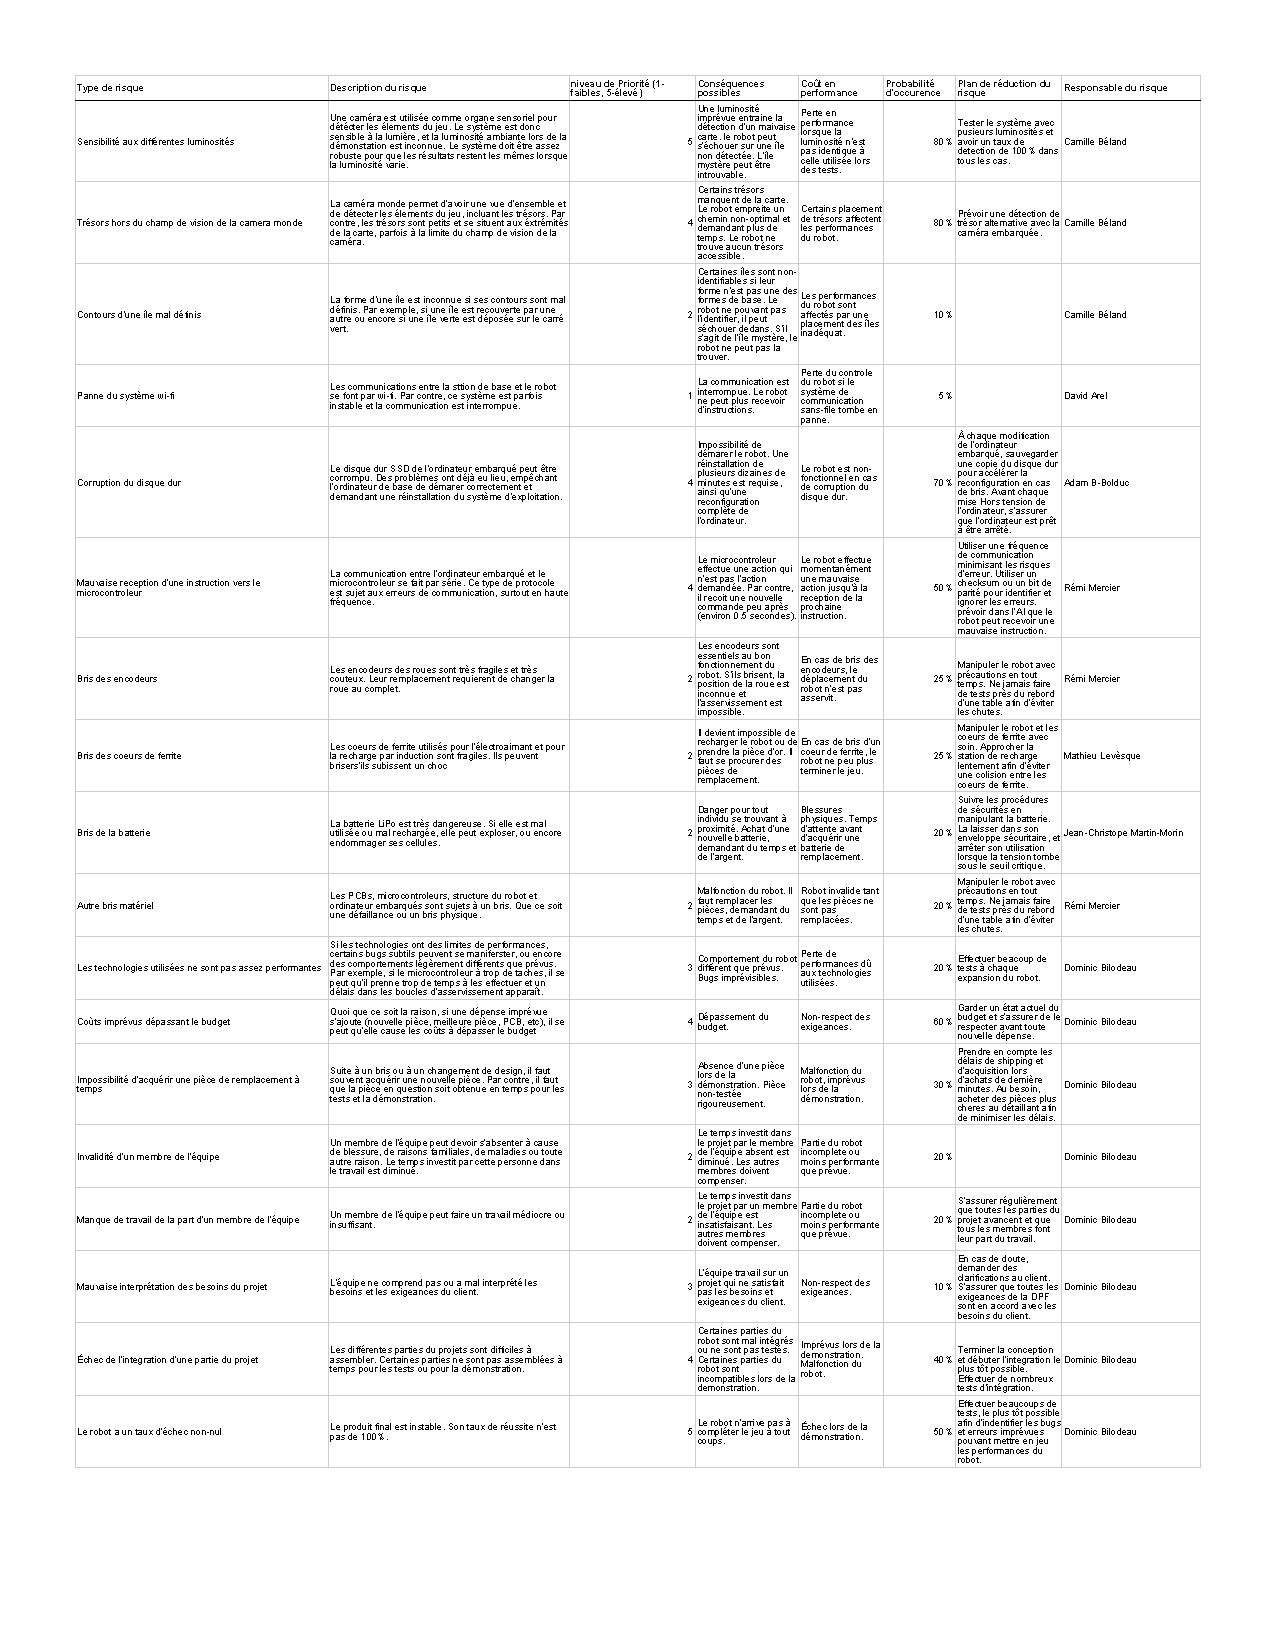
\includegraphics[scale=0.80, angle=0]{resources/risques.pdf}
\end{figure}

\chapter{Avancement de la construction système}

\section{Tests}
La partie logicielle comporte bien sûr des tests unitaires qui assurent la maintenabilité et la clareté du code.
Les tests fonctionnels peuvent être effectués à l'aide d'un simulateur qui remplace le robot physique.
On peut paramétrer ce simulateur afin qu'il induise du bruit dans le système et soit donc ainsi plus difficile à contrôler.
Ce simulateur est contrôlé par la vraie interface utilisateur du système.
Il suffit de changer le robot dans un fichier de configuration.
Ce fichier de configuration nous permet d'injecter différentes composantes selon le contexte d'exécution.

\section{Interface}
Afin d'obtenir une interface modulaire et la plus polyvalente possible nous avons opté pour une interface web.
Une composante de notre système s'occupe donc de servir les fichiers nécessaires à l'application web.
Celle-ci communique par HTTP REST ou par socket aux autres composantes du système.
La communication par socket est utilisée lorque nous avons besoin d'une boucle de rétroaction rapide,
comme dans le cas de l'information de position du robot.
La section représentant le monde de jeu de l'interface peut afficher beaucoup d'informations.
Afin de ne pas la surcharger, nous avons opté pour que chacun des affichages soit optionnel et puisse donc
être ajouté ou enlevé indépendamment, formant ainsi différentes couches.
Du point de vue des technologies, nous avons utilisé Bootstrap et AngularJS de manière à construire rapidement.
Pour dessiner les différents éléments de la carte, nous utilisons EaselJS qui nous permet d'utiliser dess fonctions avancées de dessin.


\end{document}
